\chapter{Despliegue}

El despliegue de una aplicación móvil es uno de los pasos más importantes en el ciclo de desarrollo, permitiendo que la aplicación esté disponible para los usuarios finales. Esta sección describe el proceso de despliegue del frontend desarrollado con React Native y Expo. Aunque React Native permite la creación de archivos multiplataforma, para descargar el archivo de iOS es necesario tener una cuenta de desarrollador con un coste anual, mientras que la creación del APK de Android es gratuita y es el dispositivo que tengo disponible, por lo que se describirá este proceso para obtener el APK.

Para el despliegue se hizo uso de la herramienta EAS(Expo Application Services) Build que es un servicio alojado que facilita la creación de binarios de aplicaciones para proyectos de Expo y React Native. Automatiza la construcción y distribución de aplicaciones, maneja credenciales de firma de apps, y permite compartir compilaciones internamente \cite{easbuild}.

\section{Despliegue APK}

\begin{enumerate}
    \item \textbf{Preparación del Entorno: } Para preparar el entorno de desarrollo, es necesario asegurarse de tener instalados Node.js, npm y Expo CLI. Configurar el entorno de desarrollo con las dependencias necesarias para React Native y Expo.
    \item \textbf{Configuración del Proyecto: } Hay que confirmar que en el archivo \texttt{app.json} todas las pantallas y su navegación estén correctamente configuradas para evitar problemas al tener la app instalada
    \item \textbf{Construcción del APK: } Para iniciar el proceso de construcción del APK, ejecuta el comando \texttt{expo build
          }. Expo se encargará de crear un archivo binario para Android que puede ser instalado en dispositivos Android.

\end{enumerate}

\section{Servidor}

El servidor, que incluye la API y la base de datos, se ejecutará localmente en el portátil donde se ha desarrollado la aplicación. Para el correcto funcionamiento junto con la aplicación móvil, es necesario que ambos dispositivos estén conectados a la misma red. Además, se deben habilitar los puertos y permisos necesarios en el firewall del portátil para aceptar las peticiones HTTP realizadas por la aplicación móvil.

\section{HangOut}

A continuación se mostrarán capturas de las diferentes pantallas de la aplicación y se incluirá un enlace a los vídeos que demuestran su correcto funcionamiento y la navegación entre sus páginas:

\clearpage
\vspace*{\fill}
\begin{figure}[H]
    \centering
    \begin{subfigure}{0.45\textwidth}
        \centering
        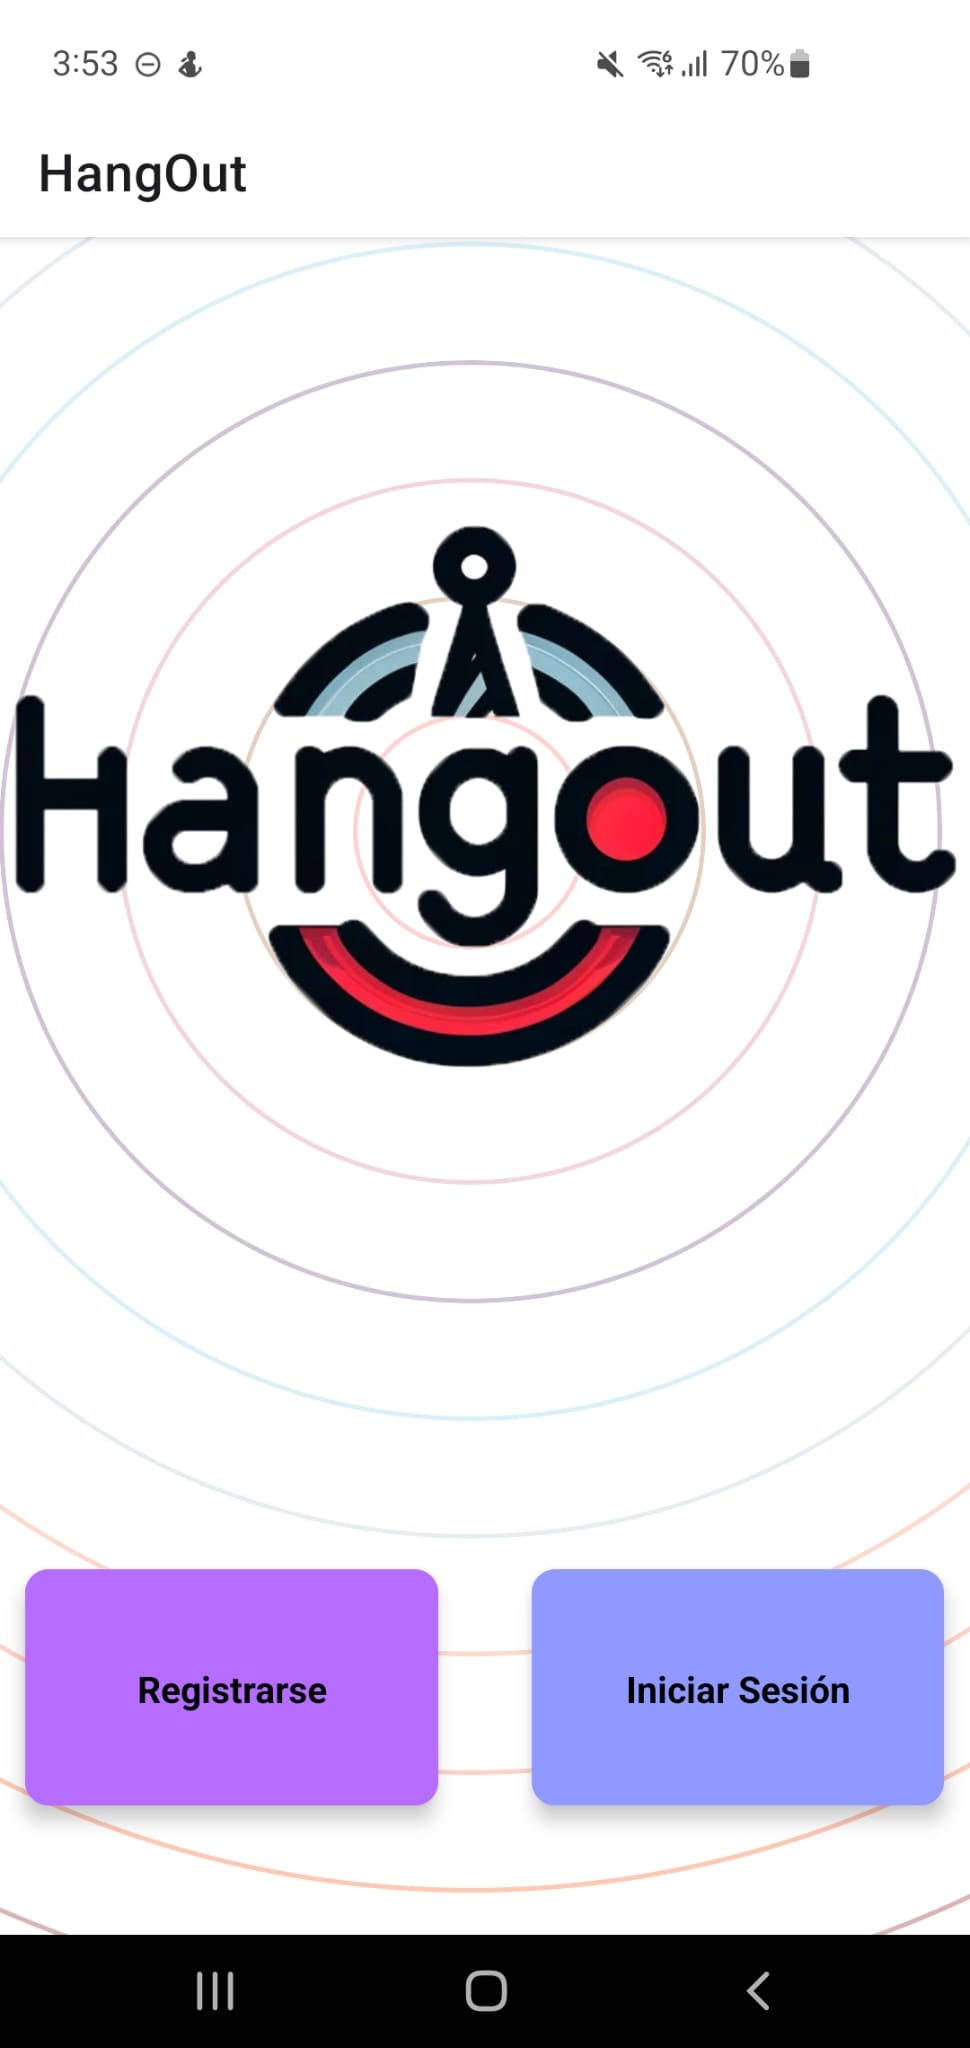
\includegraphics[width=\linewidth]{imagenes/Capturas/Inicio.jpeg}
        \caption{Inicio de la aplicación}
        \label{fig:img5}
    \end{subfigure}%
    \hfill
    \begin{subfigure}{0.45\textwidth}
        \centering
        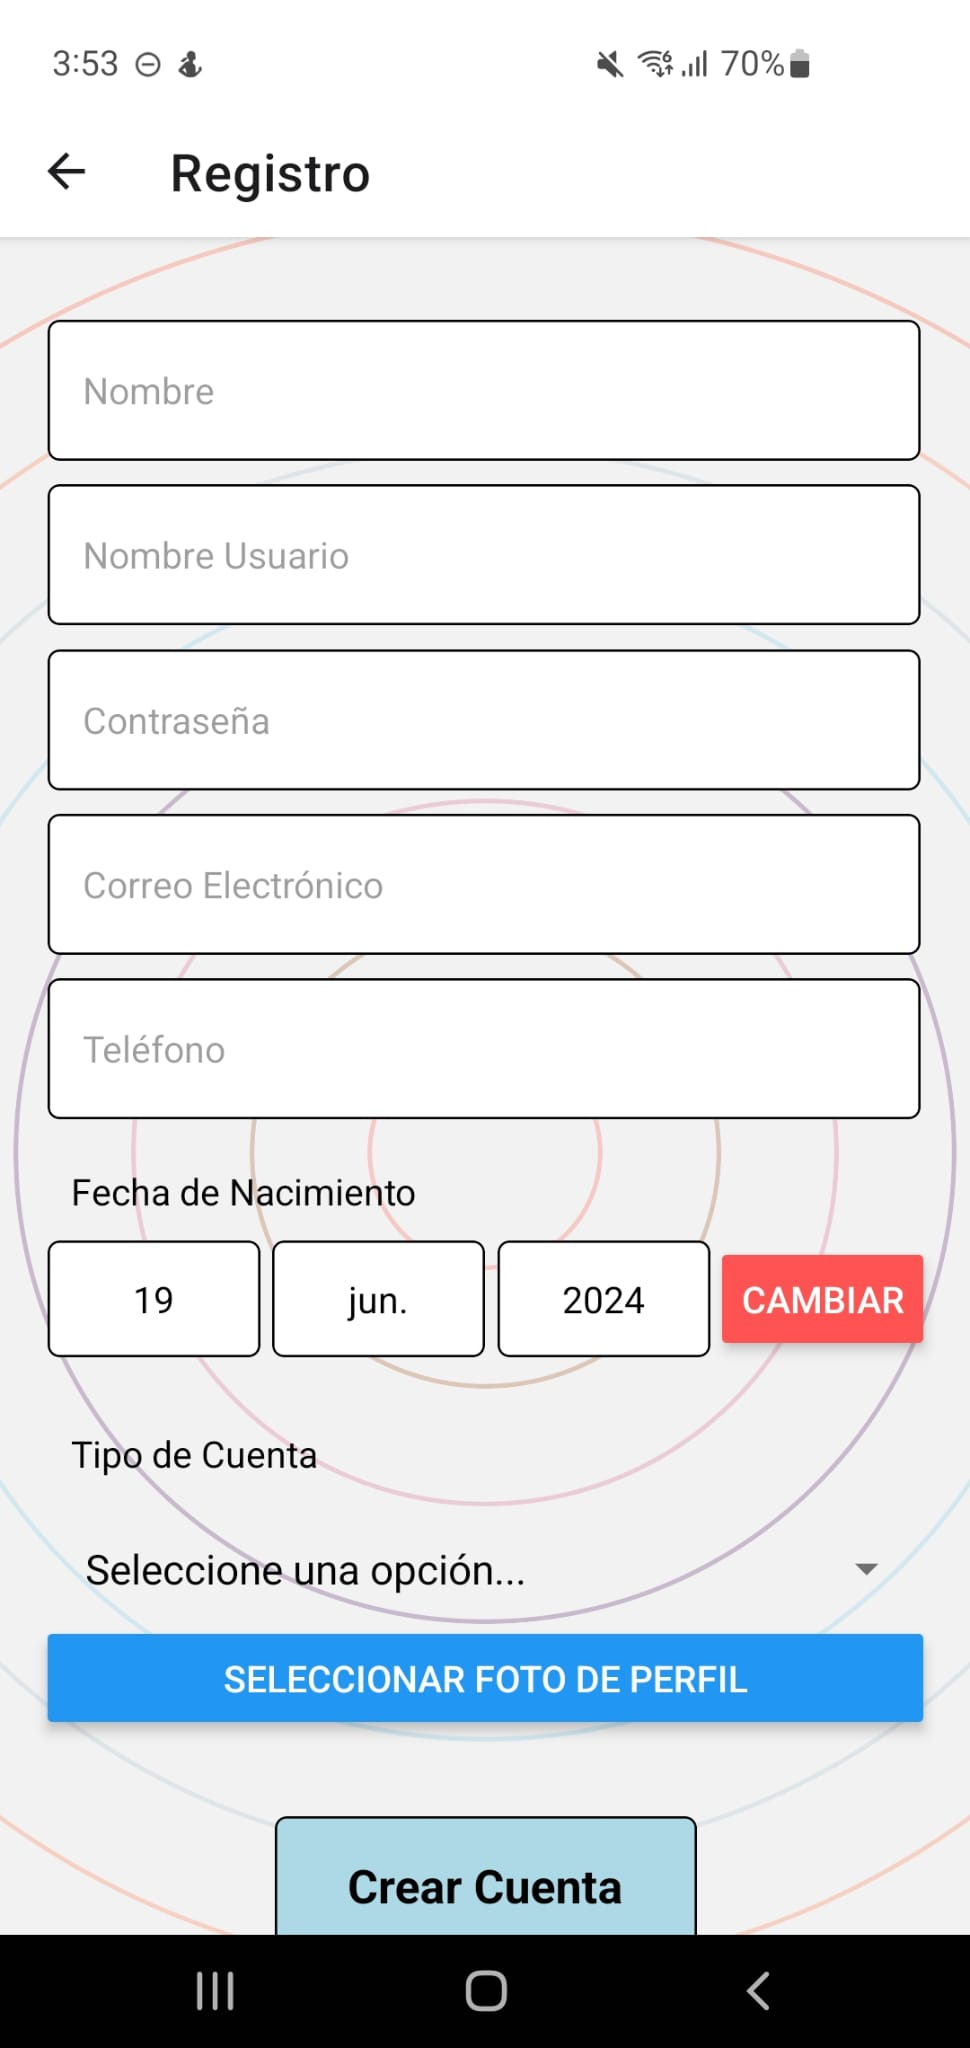
\includegraphics[width=\linewidth]{imagenes/Capturas/Registro.jpeg}
        \caption{Registro}
        \label{fig:img6}
    \end{subfigure}
\end{figure}
\vspace*{\fill}

\clearpage
\vspace*{\fill}
\begin{figure}[H]
    \centering
    \begin{subfigure}{0.45\textwidth}
        \centering
        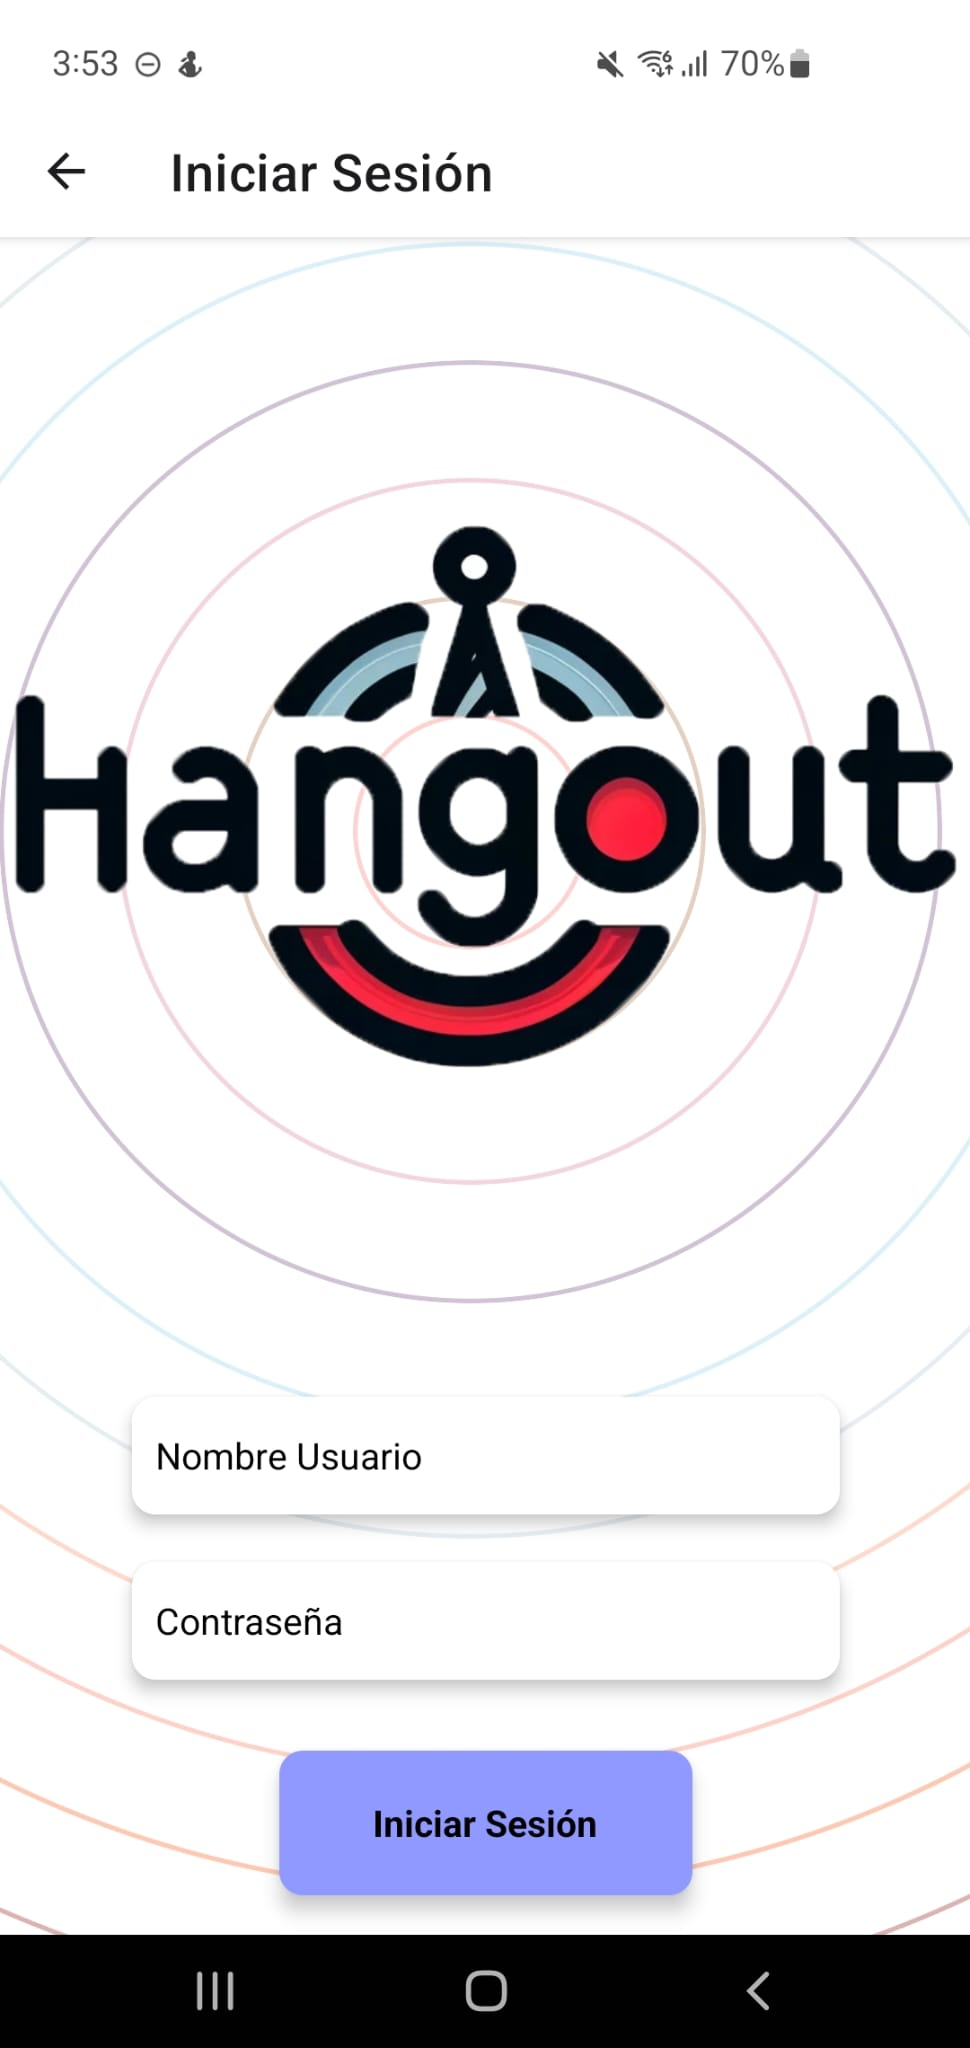
\includegraphics[width=\linewidth]{imagenes/Capturas/InicioSesion.jpeg}
        \caption{Inicio Sesión}
        \label{fig:img5}
    \end{subfigure}%
    \hfill
    \begin{subfigure}{0.45\textwidth}
        \centering
        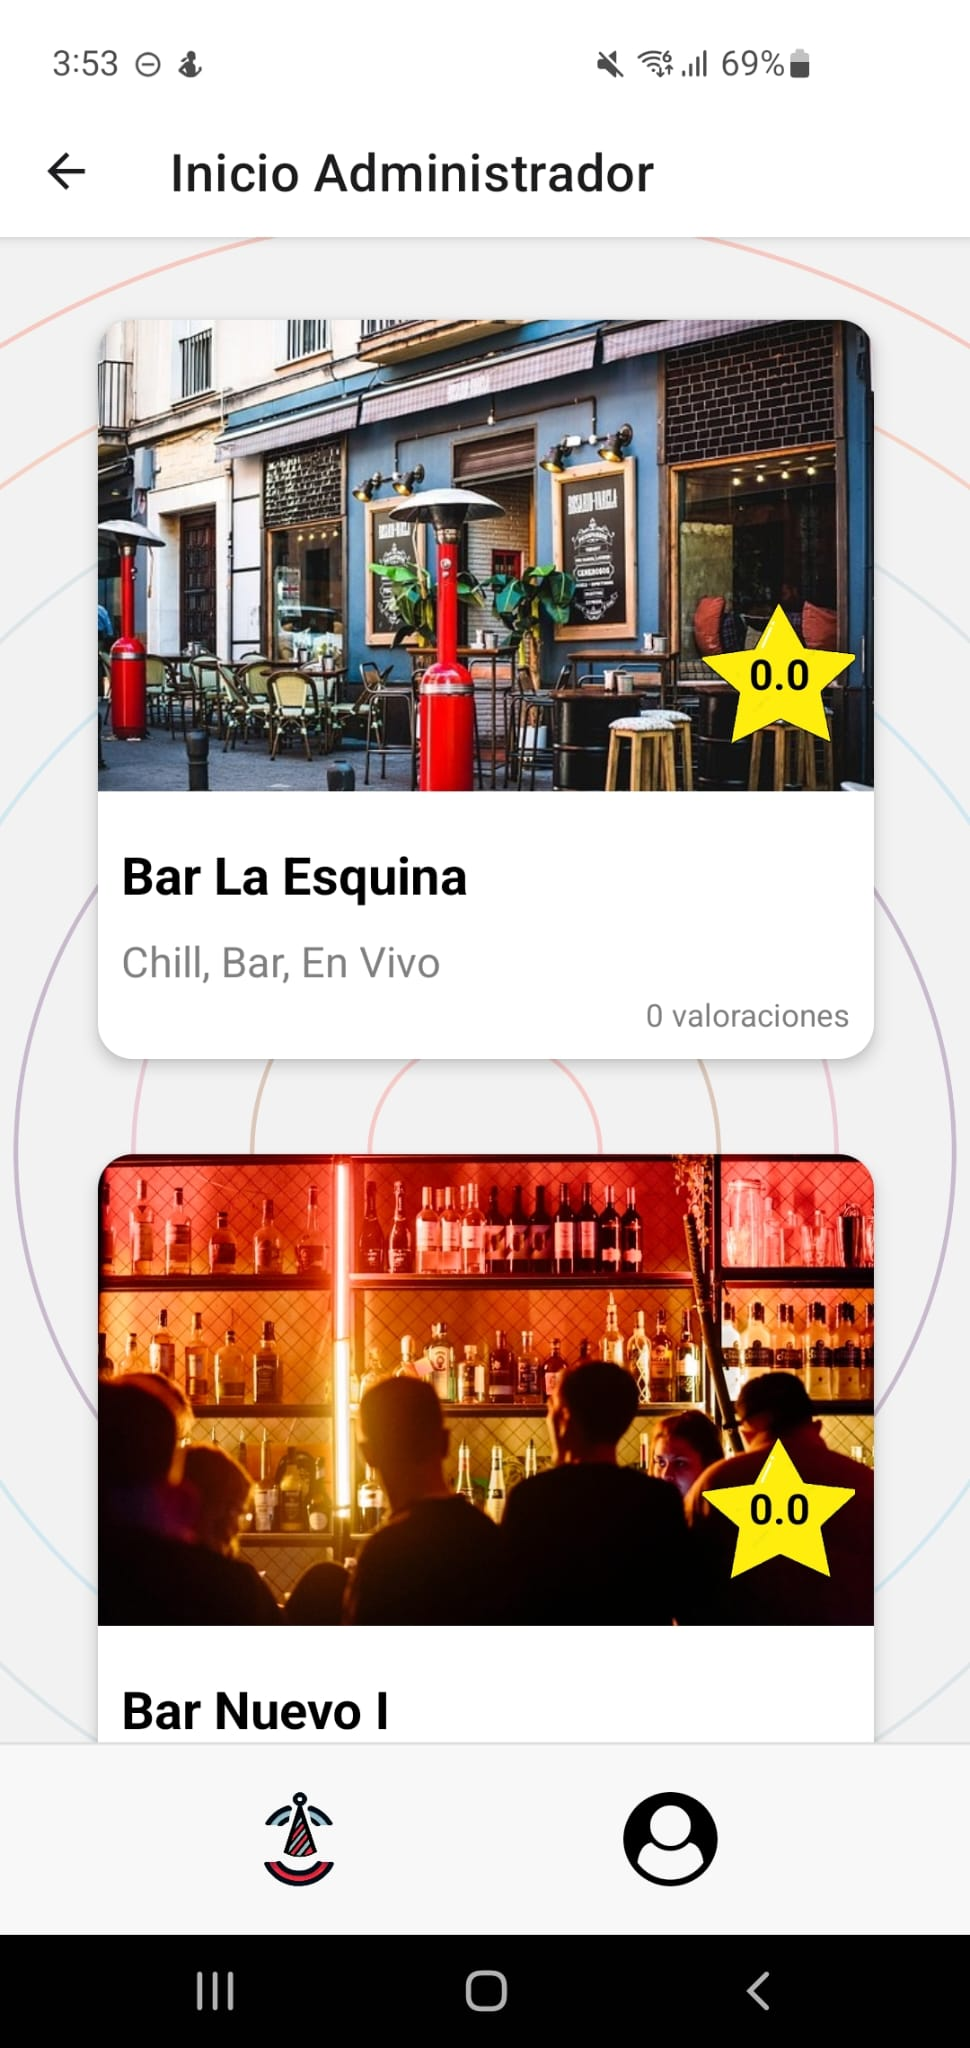
\includegraphics[width=\linewidth]{imagenes/Capturas/InicioAdmin.jpeg}
        \caption{Pantalla Inicio Administrador}
        \label{fig:img6}
    \end{subfigure}
\end{figure}
\vspace*{\fill}

\clearpage
\vspace*{\fill}
\begin{figure}[H]
    \centering
    \begin{subfigure}{0.45\textwidth}
        \centering
        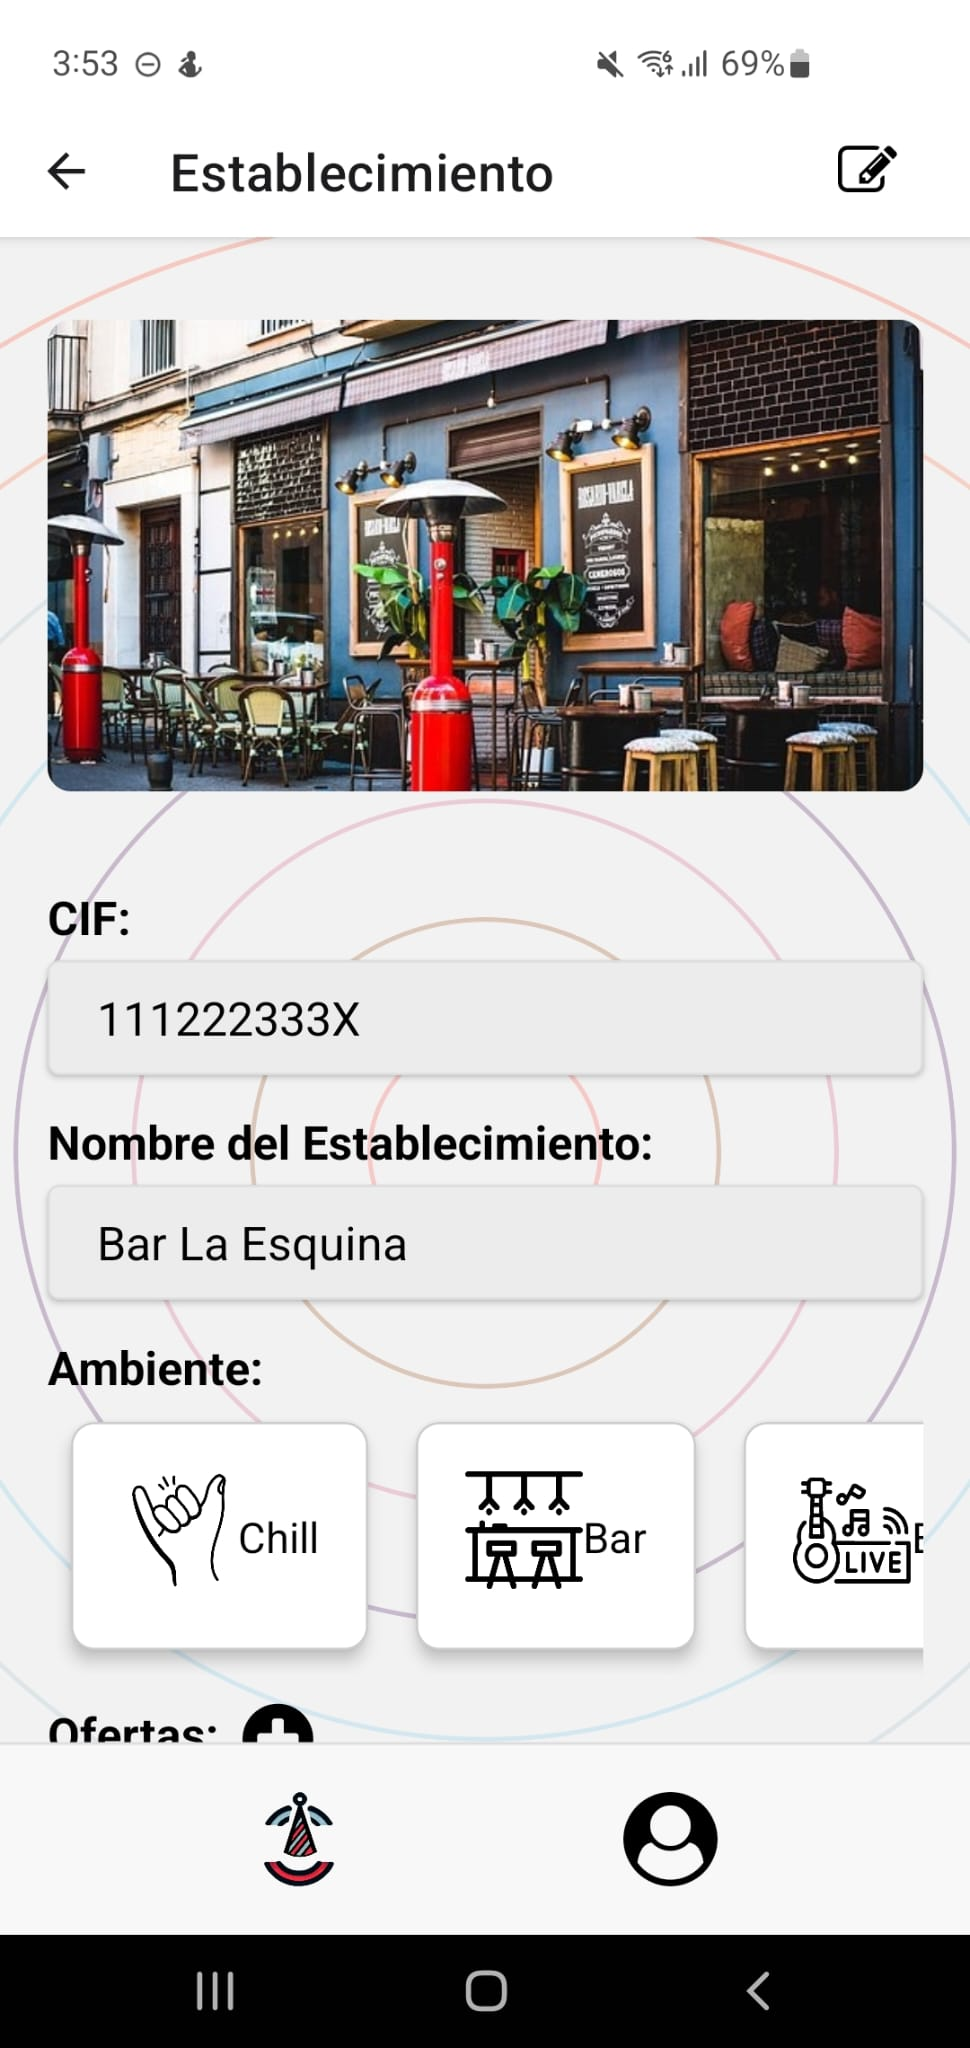
\includegraphics[width=\linewidth]{imagenes/Capturas/DatosEstablecimiento.jpeg}
        \caption{Datos Establecimiento}
        \label{fig:img5}
    \end{subfigure}%
    \hfill
    \begin{subfigure}{0.45\textwidth}
        \centering
        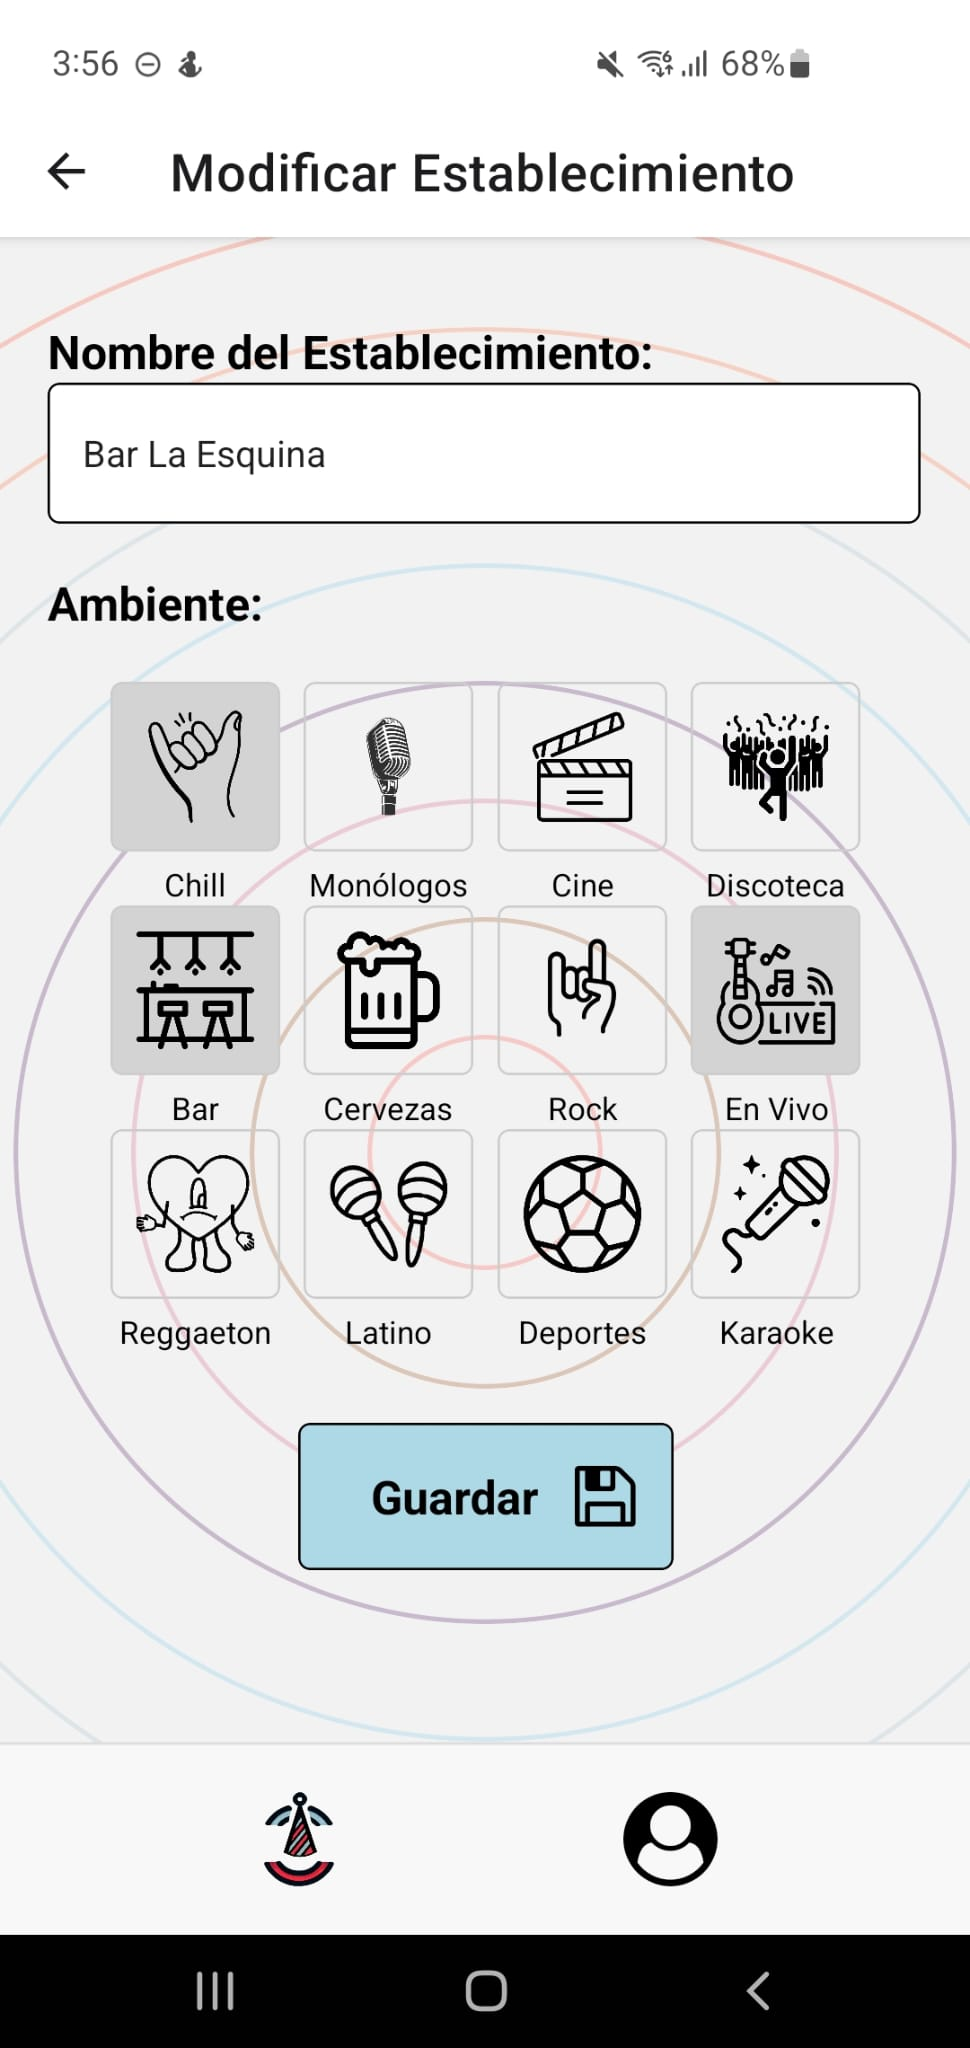
\includegraphics[width=\linewidth]{imagenes/Capturas/ModificarEstablecimiento.jpeg}
        \caption{Modificar Establecimiento}
        \label{fig:img6}
    \end{subfigure}
\end{figure}
\vspace*{\fill}

\clearpage
\vspace*{\fill}
\begin{figure}[H]
    \centering
    \begin{subfigure}{0.45\textwidth}
        \centering
        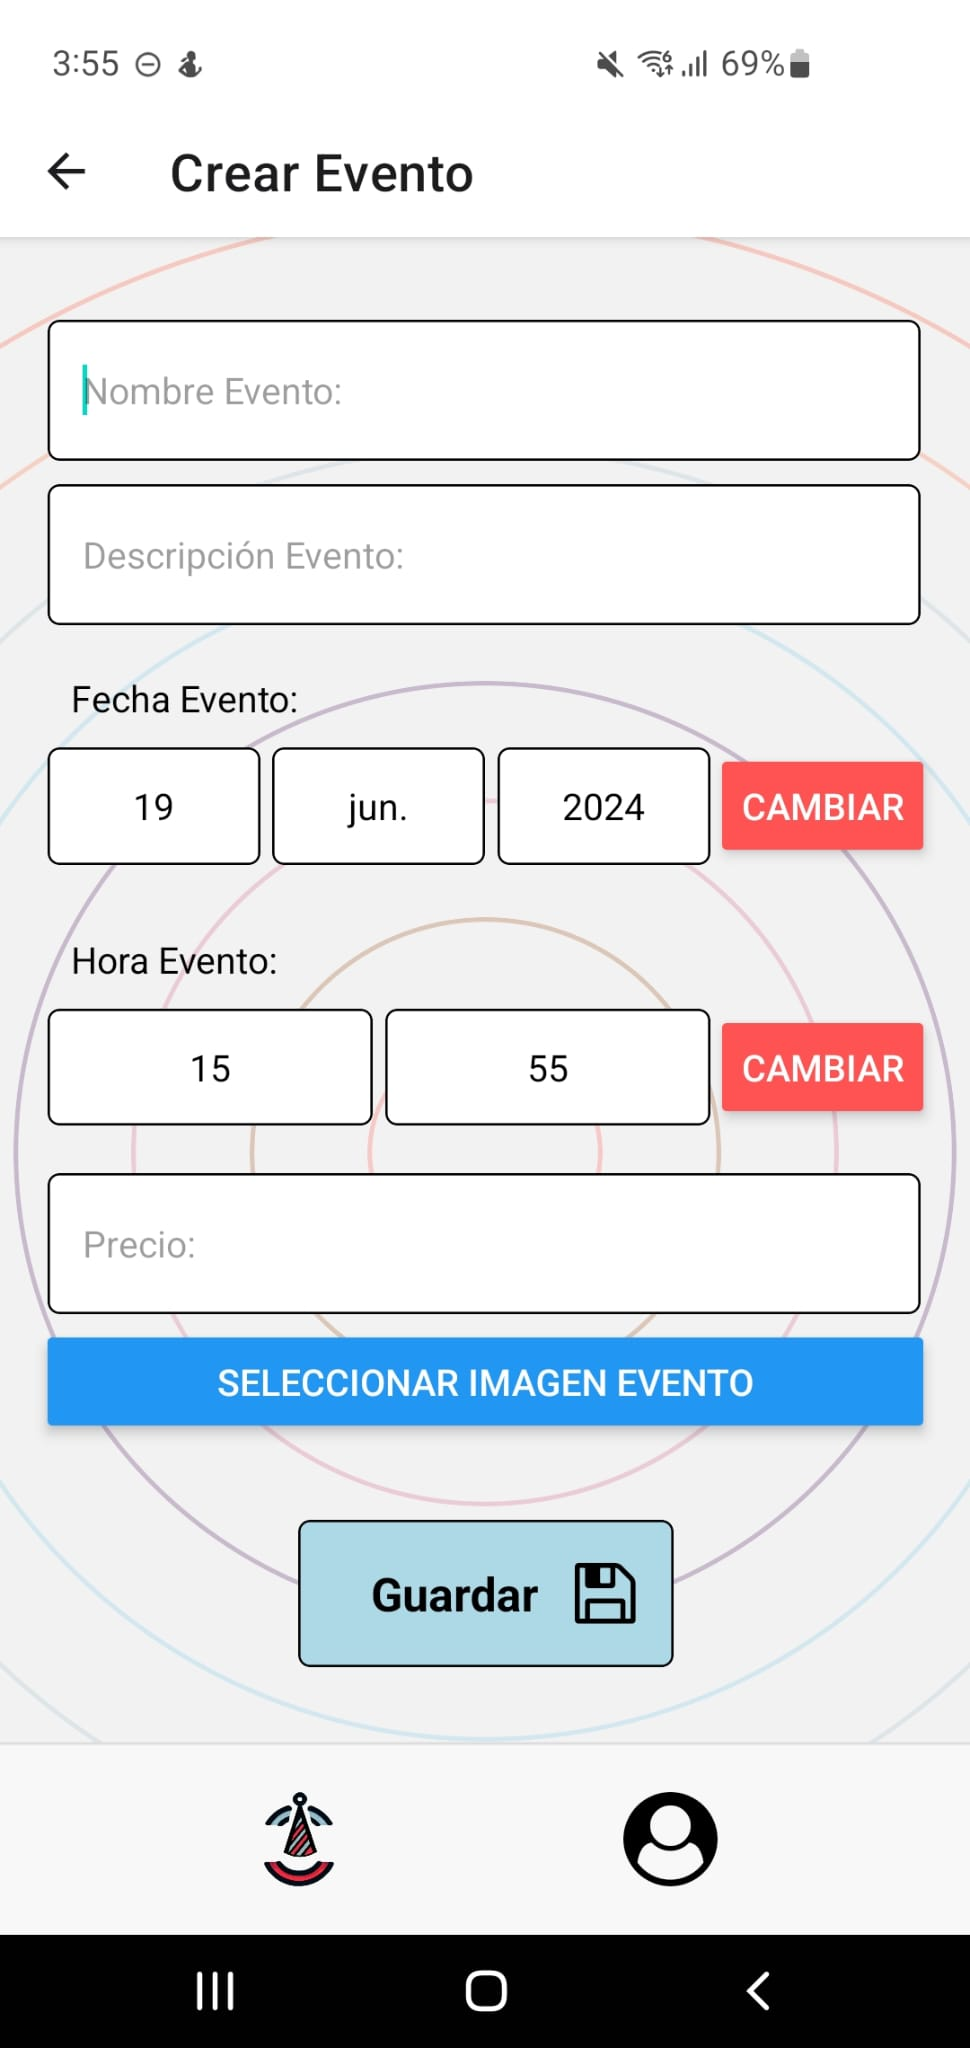
\includegraphics[width=\linewidth]{imagenes/Capturas/CrearEvento.jpeg}
        \caption{Crear Evento}
        \label{fig:img5}
    \end{subfigure}%
    \hfill
    \begin{subfigure}{0.45\textwidth}
        \centering
        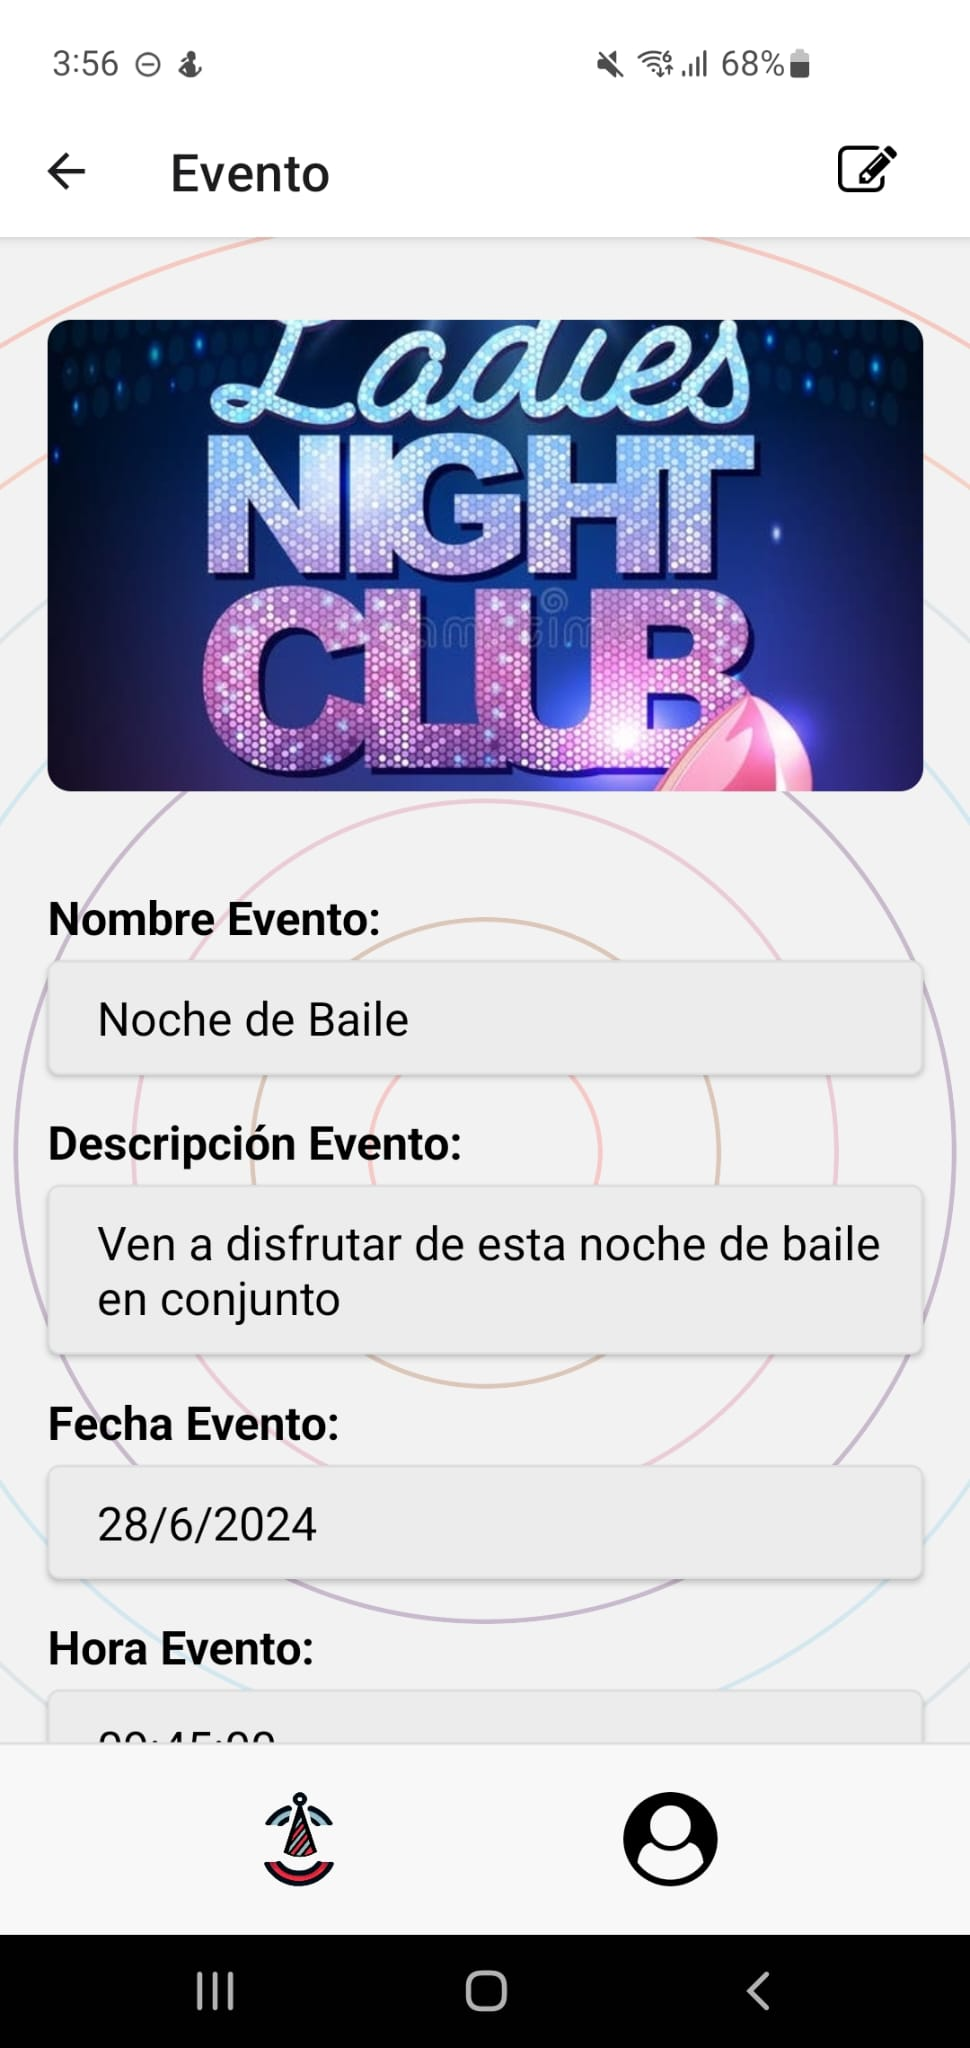
\includegraphics[width=\linewidth]{imagenes/Capturas/DatosEventoAdmin.jpeg}
        \caption{Datos del Evento}
        \label{fig:img6}
    \end{subfigure}
\end{figure}
\vspace*{\fill}

\clearpage
\vspace*{\fill}
\begin{figure}[H]
    \centering
    \begin{subfigure}{0.45\textwidth}
        \centering
        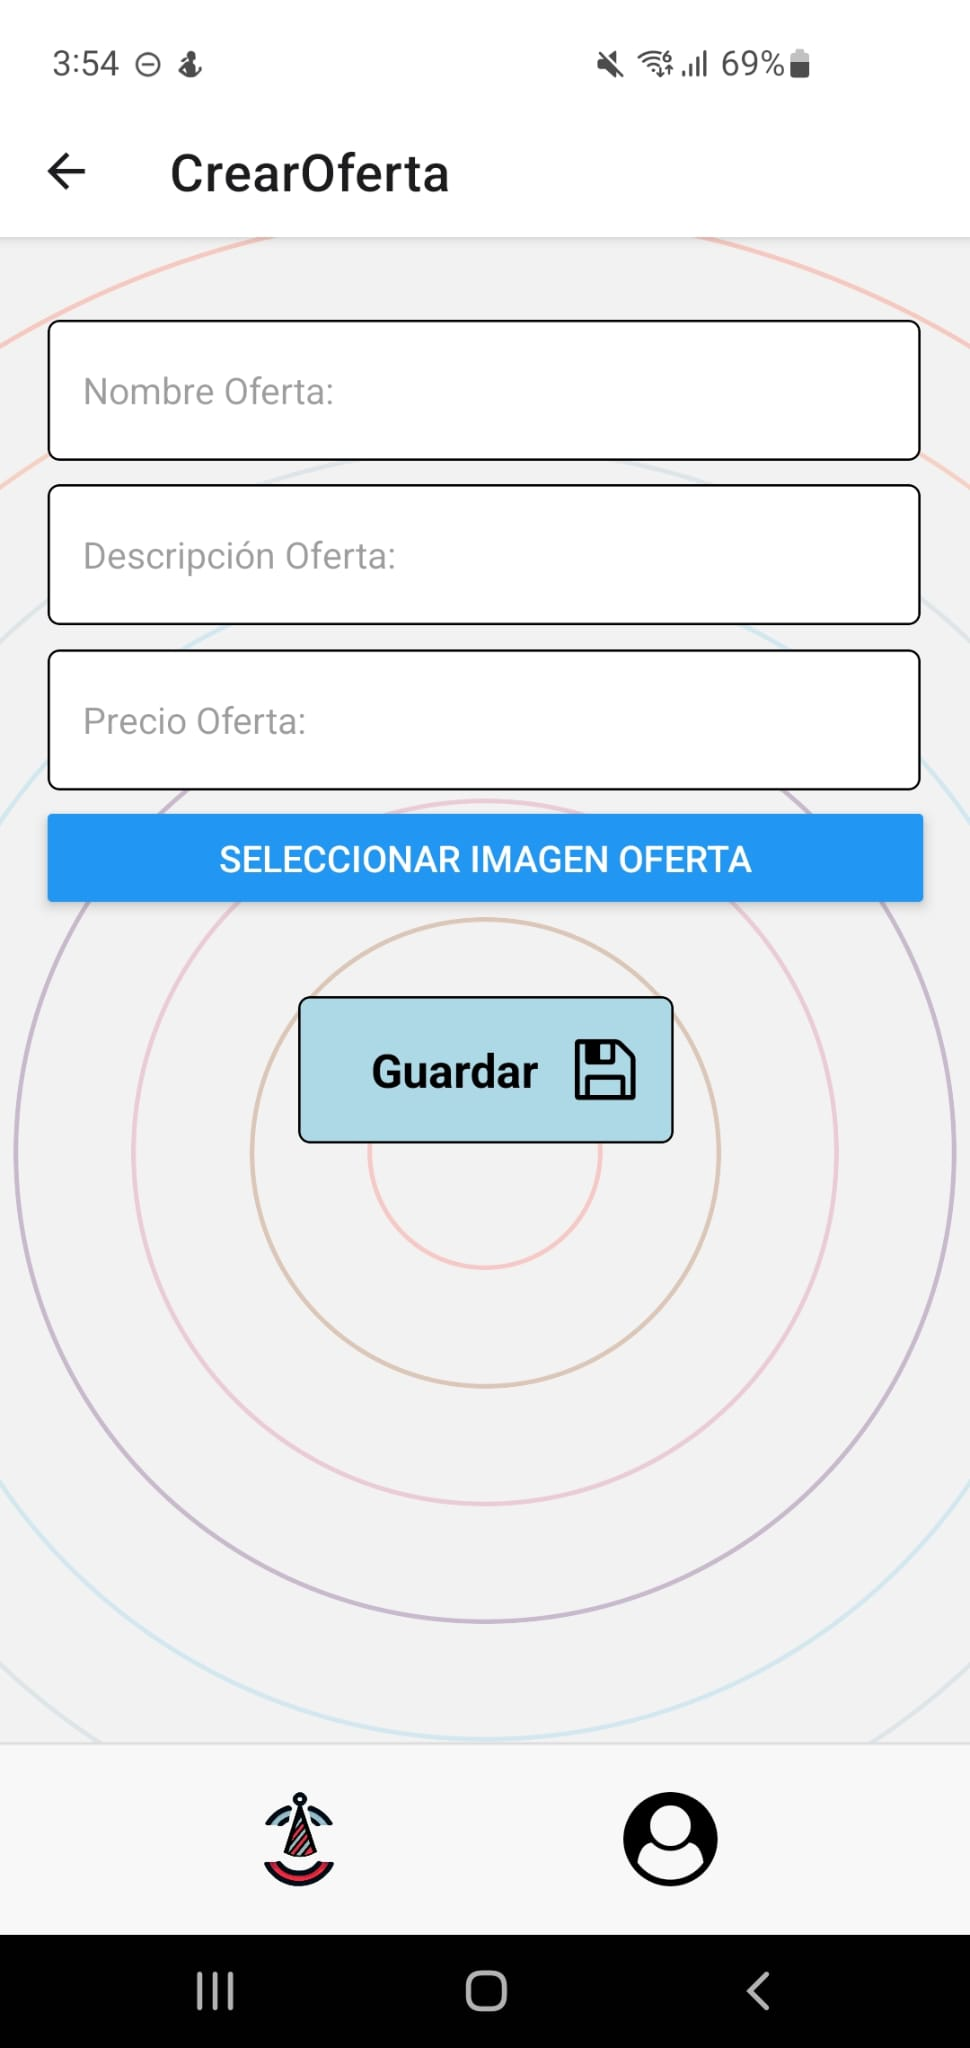
\includegraphics[width=\linewidth]{imagenes/Capturas/CrearOferta.jpeg}
        \caption{Crear Oferta}
        \label{fig:img5}
    \end{subfigure}%
    \hfill
    \begin{subfigure}{0.45\textwidth}
        \centering
        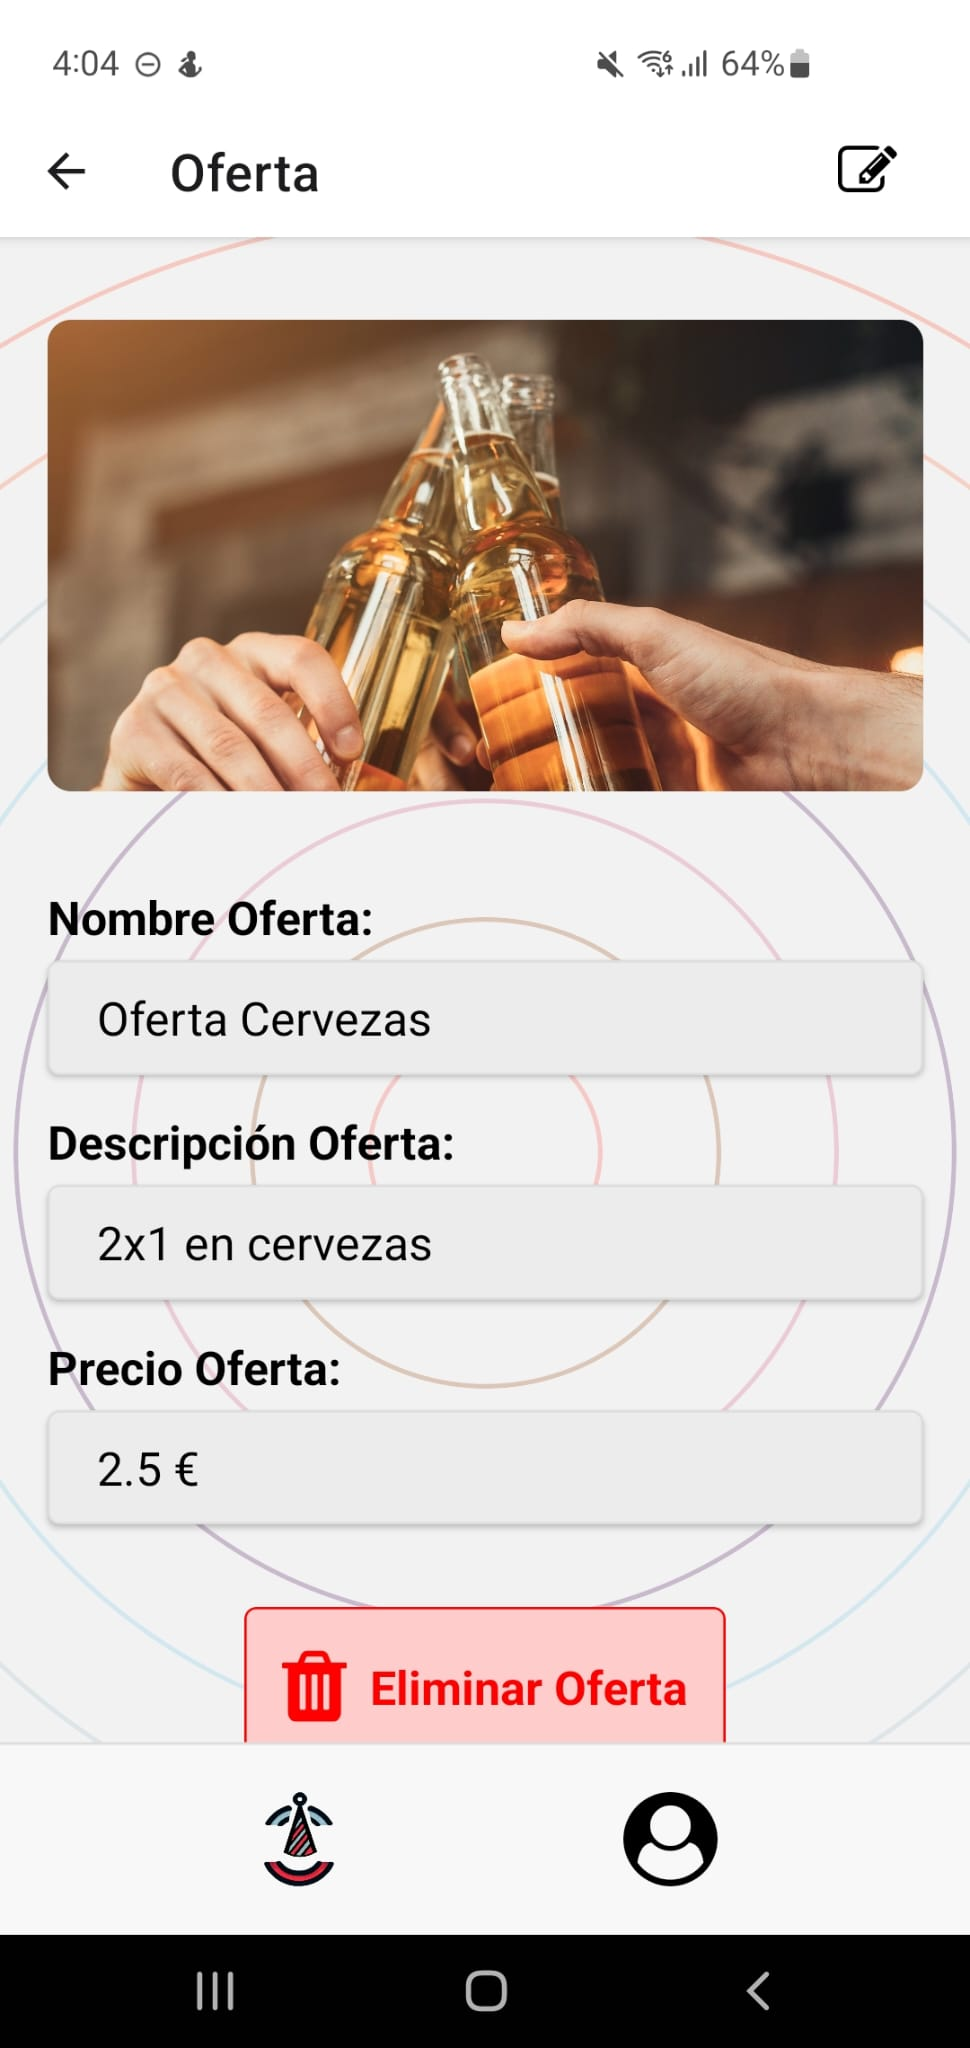
\includegraphics[width=\linewidth]{imagenes/Capturas/DatosOferta.jpeg}
        \caption{Datos de la Oferta}
        \label{fig:img6}
    \end{subfigure}
\end{figure}
\vspace*{\fill}

\clearpage
\vspace*{\fill}
\begin{figure}[H]
    \centering
    \begin{subfigure}{0.45\textwidth}
        \centering
        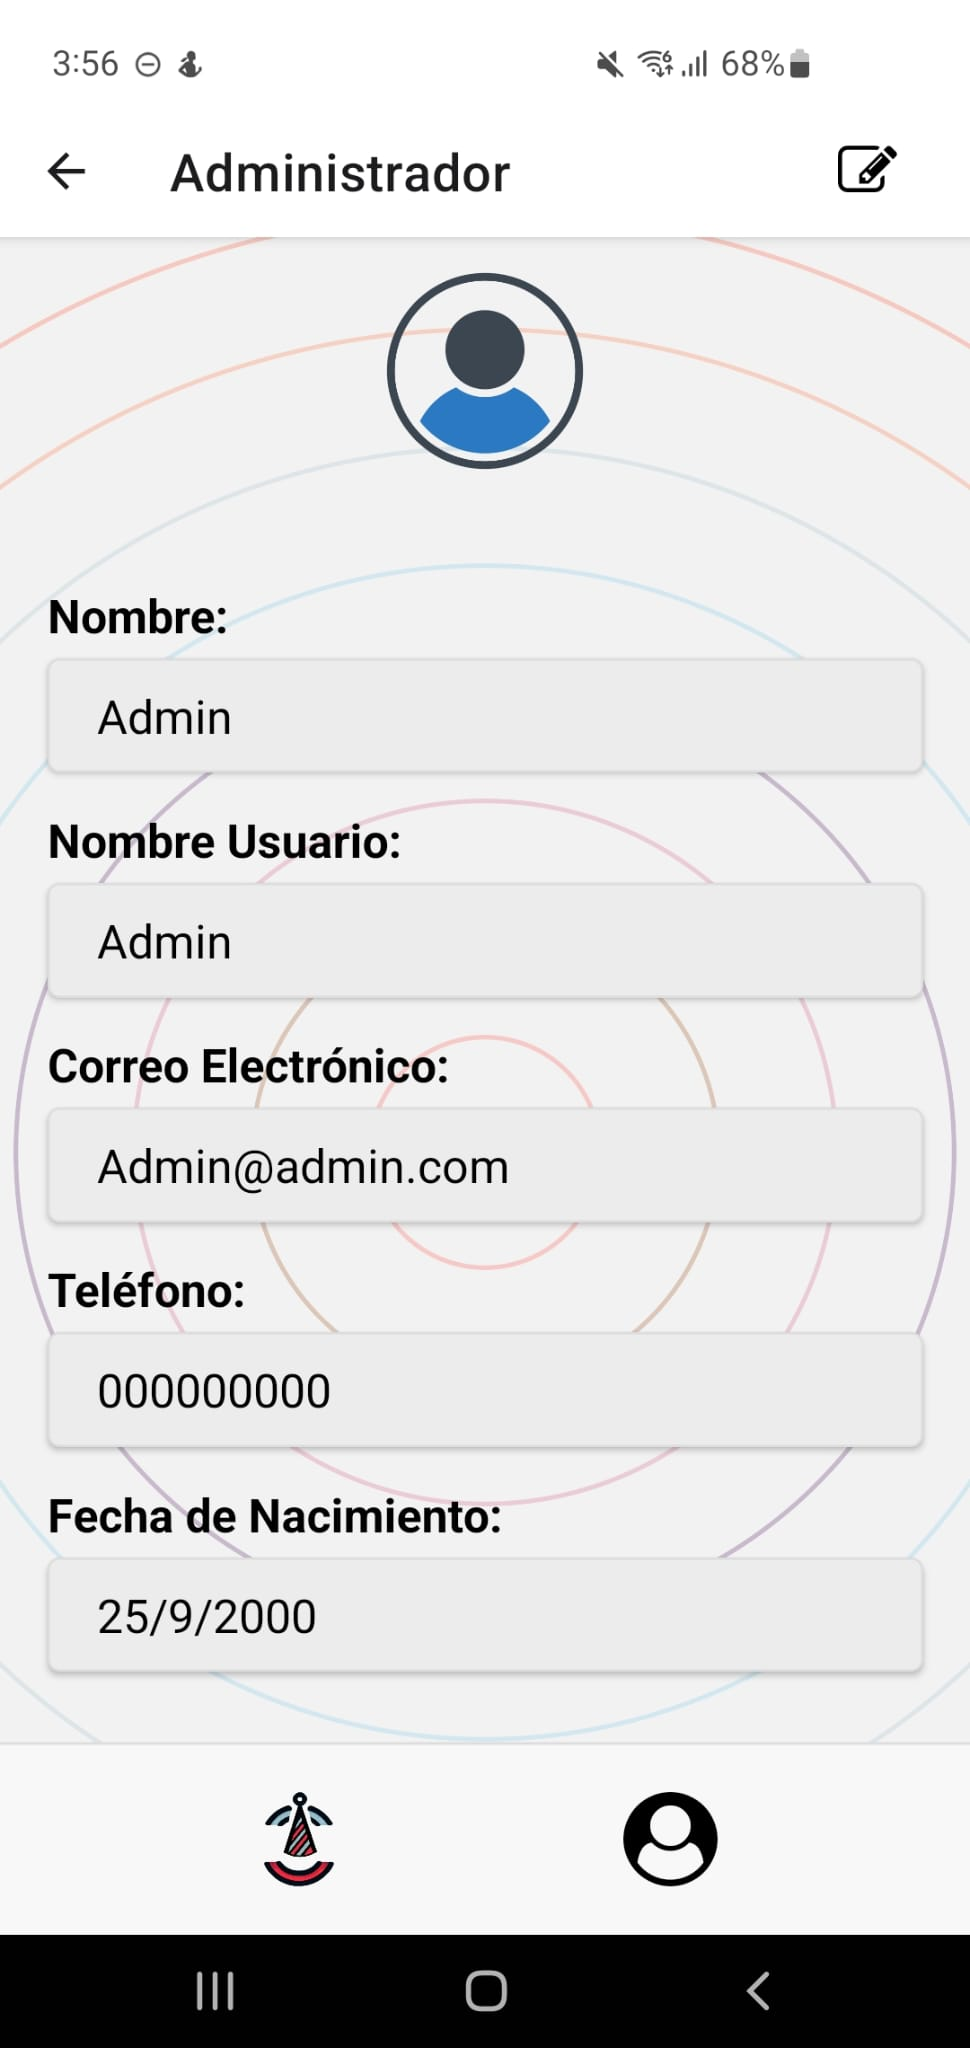
\includegraphics[width=\linewidth]{imagenes/Capturas/DatosPerfilAdmin.jpeg}
        \caption{Datos del Administrador}
        \label{fig:img5}
    \end{subfigure}%
    \hfill
    \begin{subfigure}{0.45\textwidth}
        \centering
        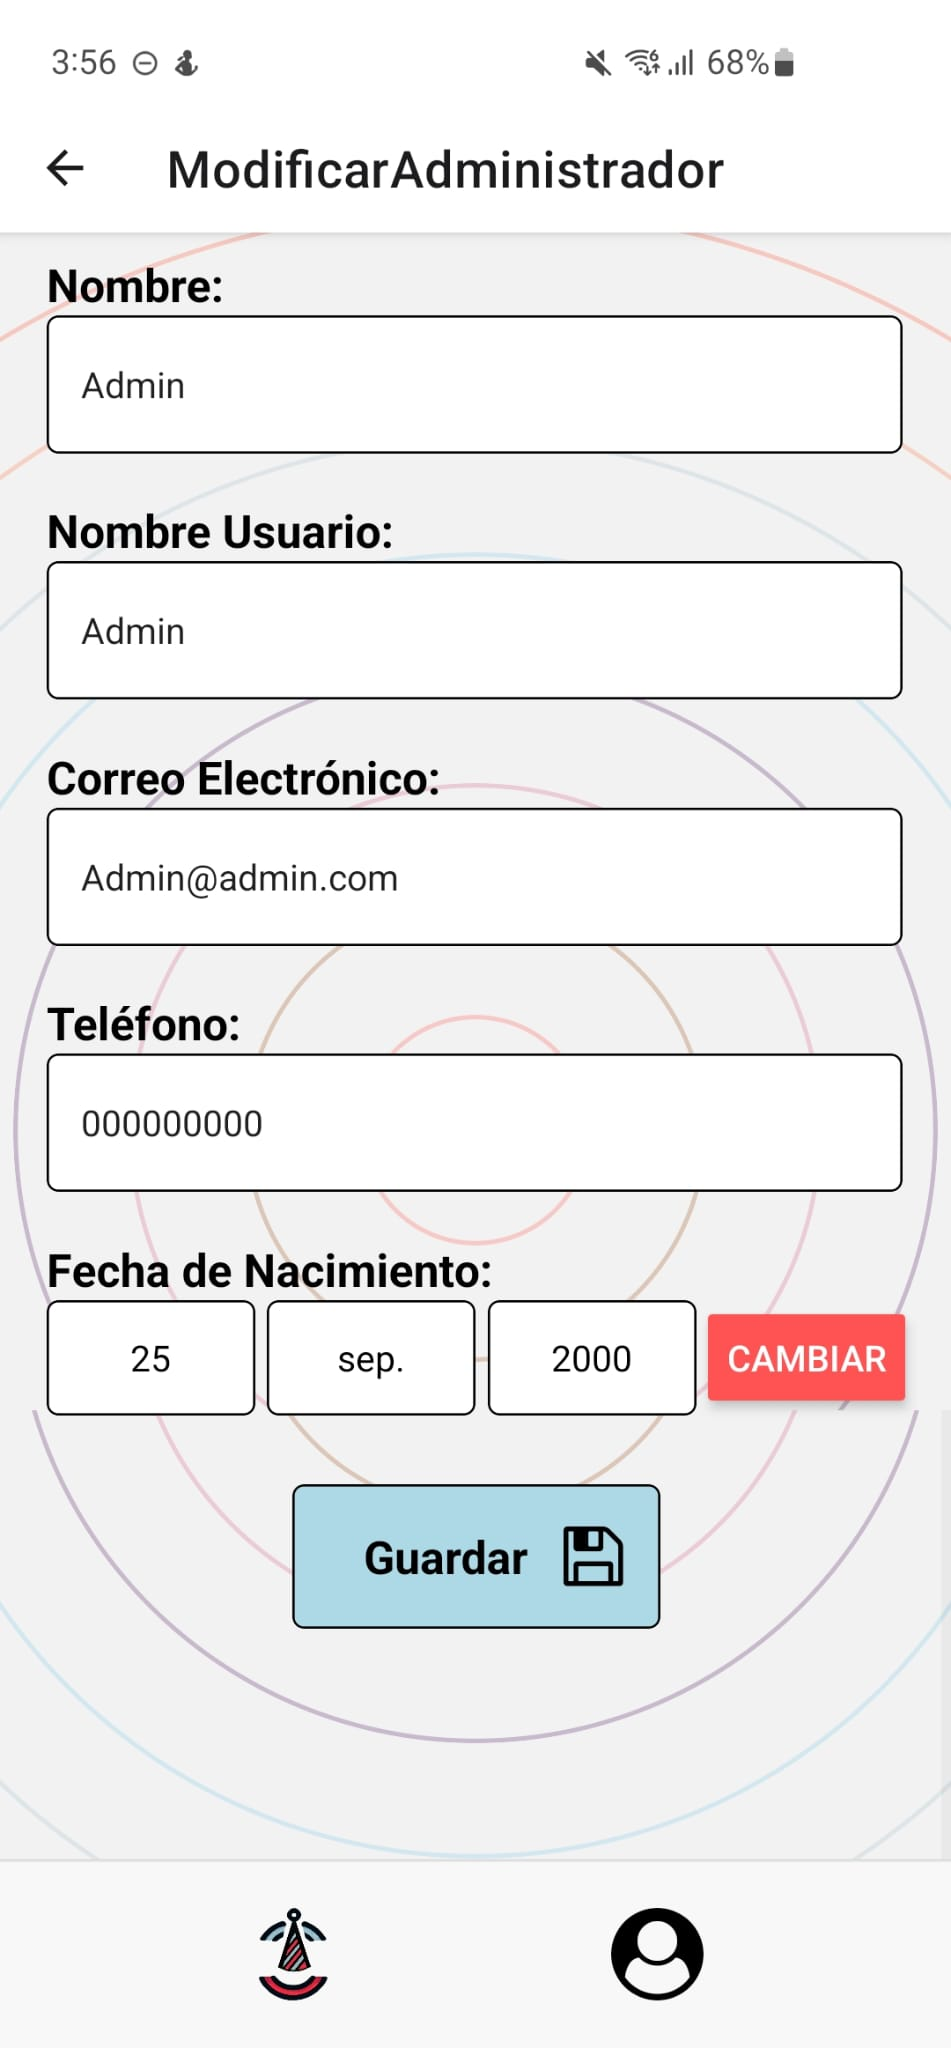
\includegraphics[width=\linewidth]{imagenes/Capturas/ModificarAdministrador.jpeg}
        \caption{Modificar Perfil Administrador}
        \label{fig:img6}
    \end{subfigure}
\end{figure}
\vspace*{\fill}

\clearpage
\vspace*{\fill}
\begin{figure}[H]
    \centering
    \begin{subfigure}{0.45\textwidth}
        \centering
        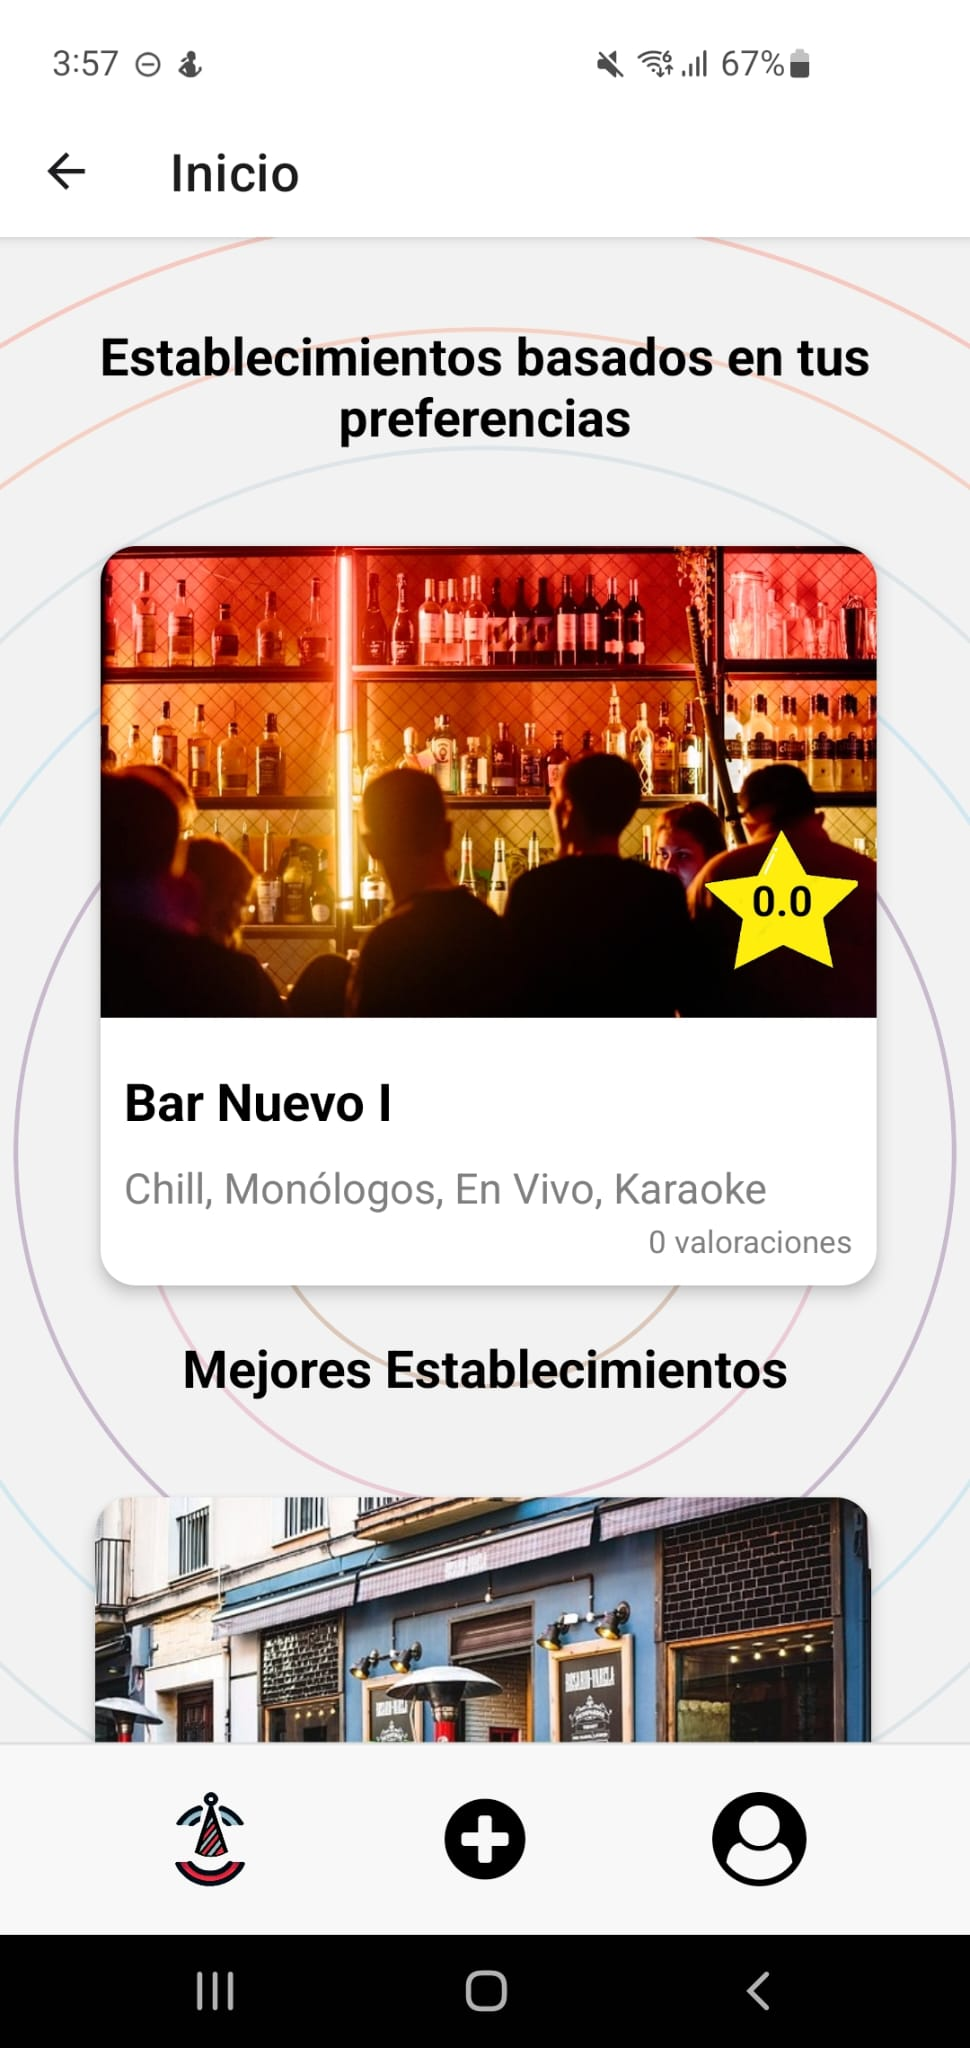
\includegraphics[width=\linewidth]{imagenes/Capturas/InicioUsuario.jpeg}
        \caption{Pantalla Inicio Usuario}
        \label{fig:img5}
    \end{subfigure}%
    \hfill
    \begin{subfigure}{0.45\textwidth}
        \centering
        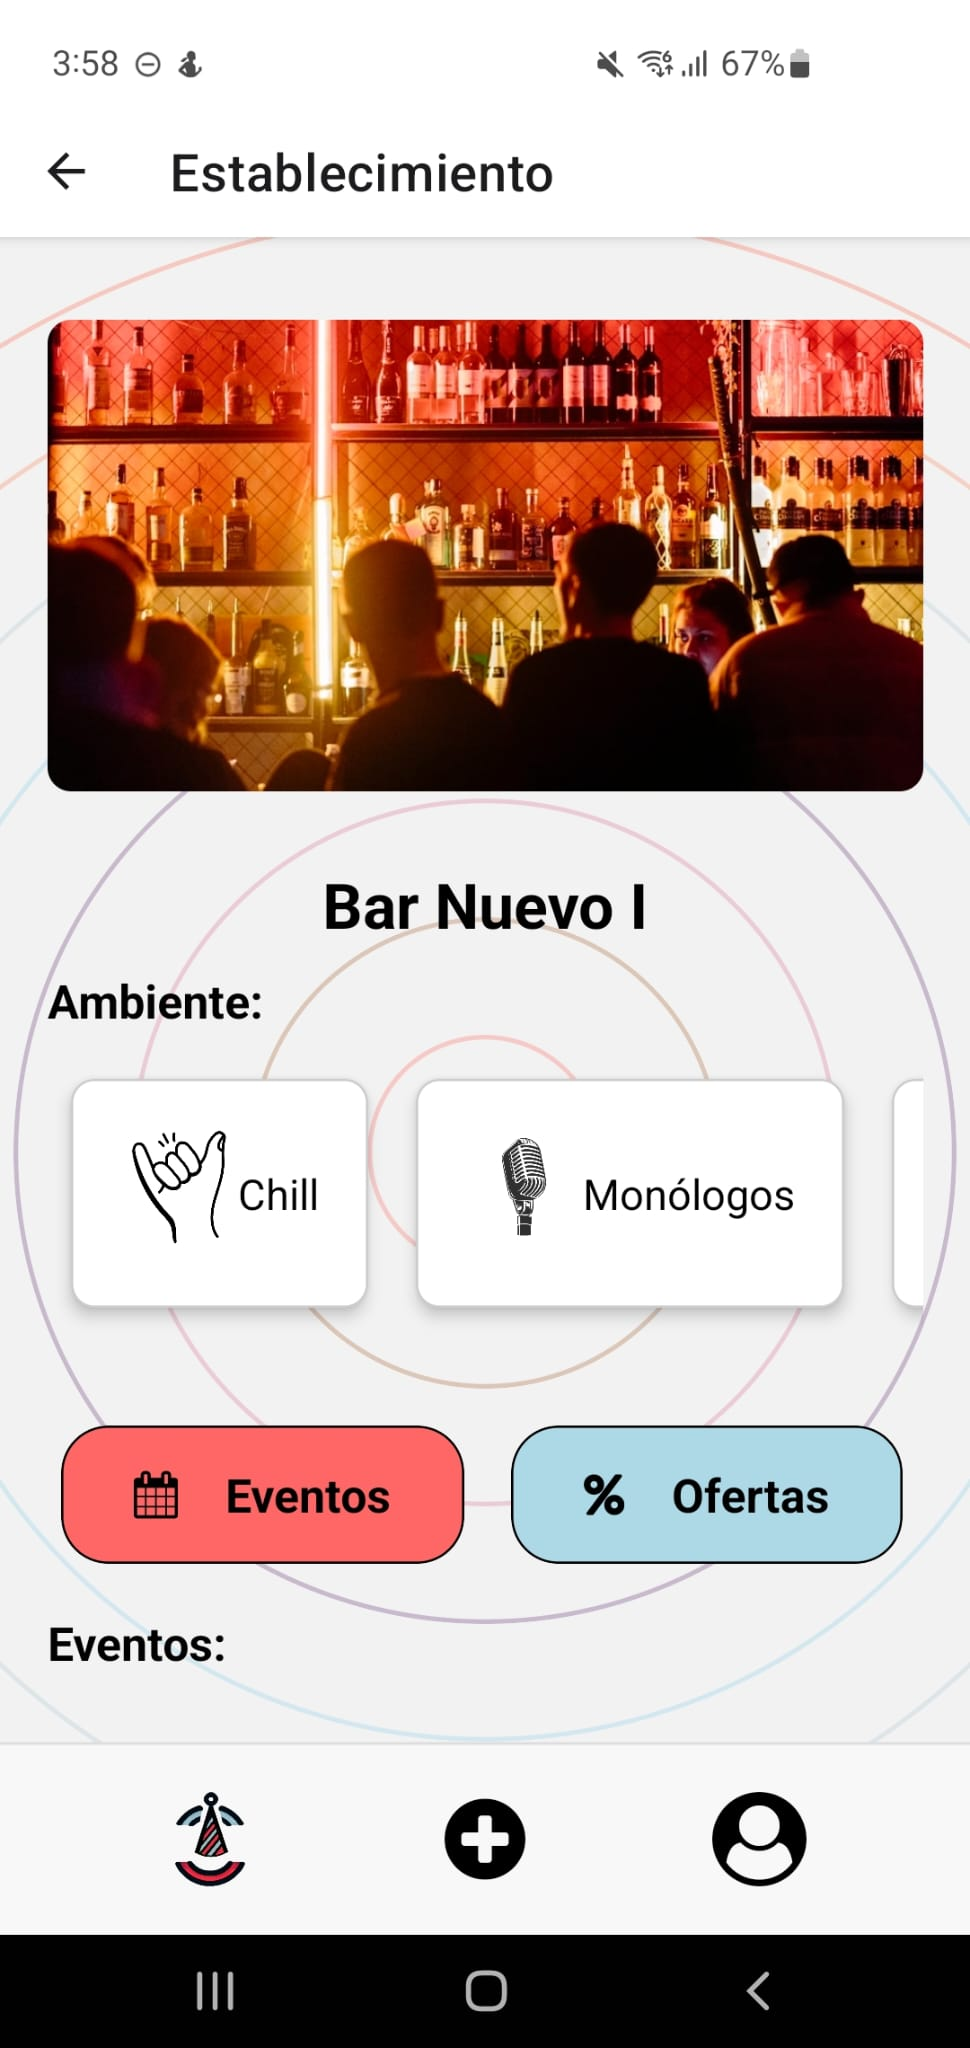
\includegraphics[width=\linewidth]{imagenes/Capturas/DatosEstablecimientoUsuario.jpeg}
        \caption{Datos del Establecimiento}
        \label{fig:img6}
    \end{subfigure}
\end{figure}
\vspace*{\fill}

\clearpage
\vspace*{\fill}
\begin{figure}[H]
    \centering
    \begin{subfigure}{0.45\textwidth}
        \centering
        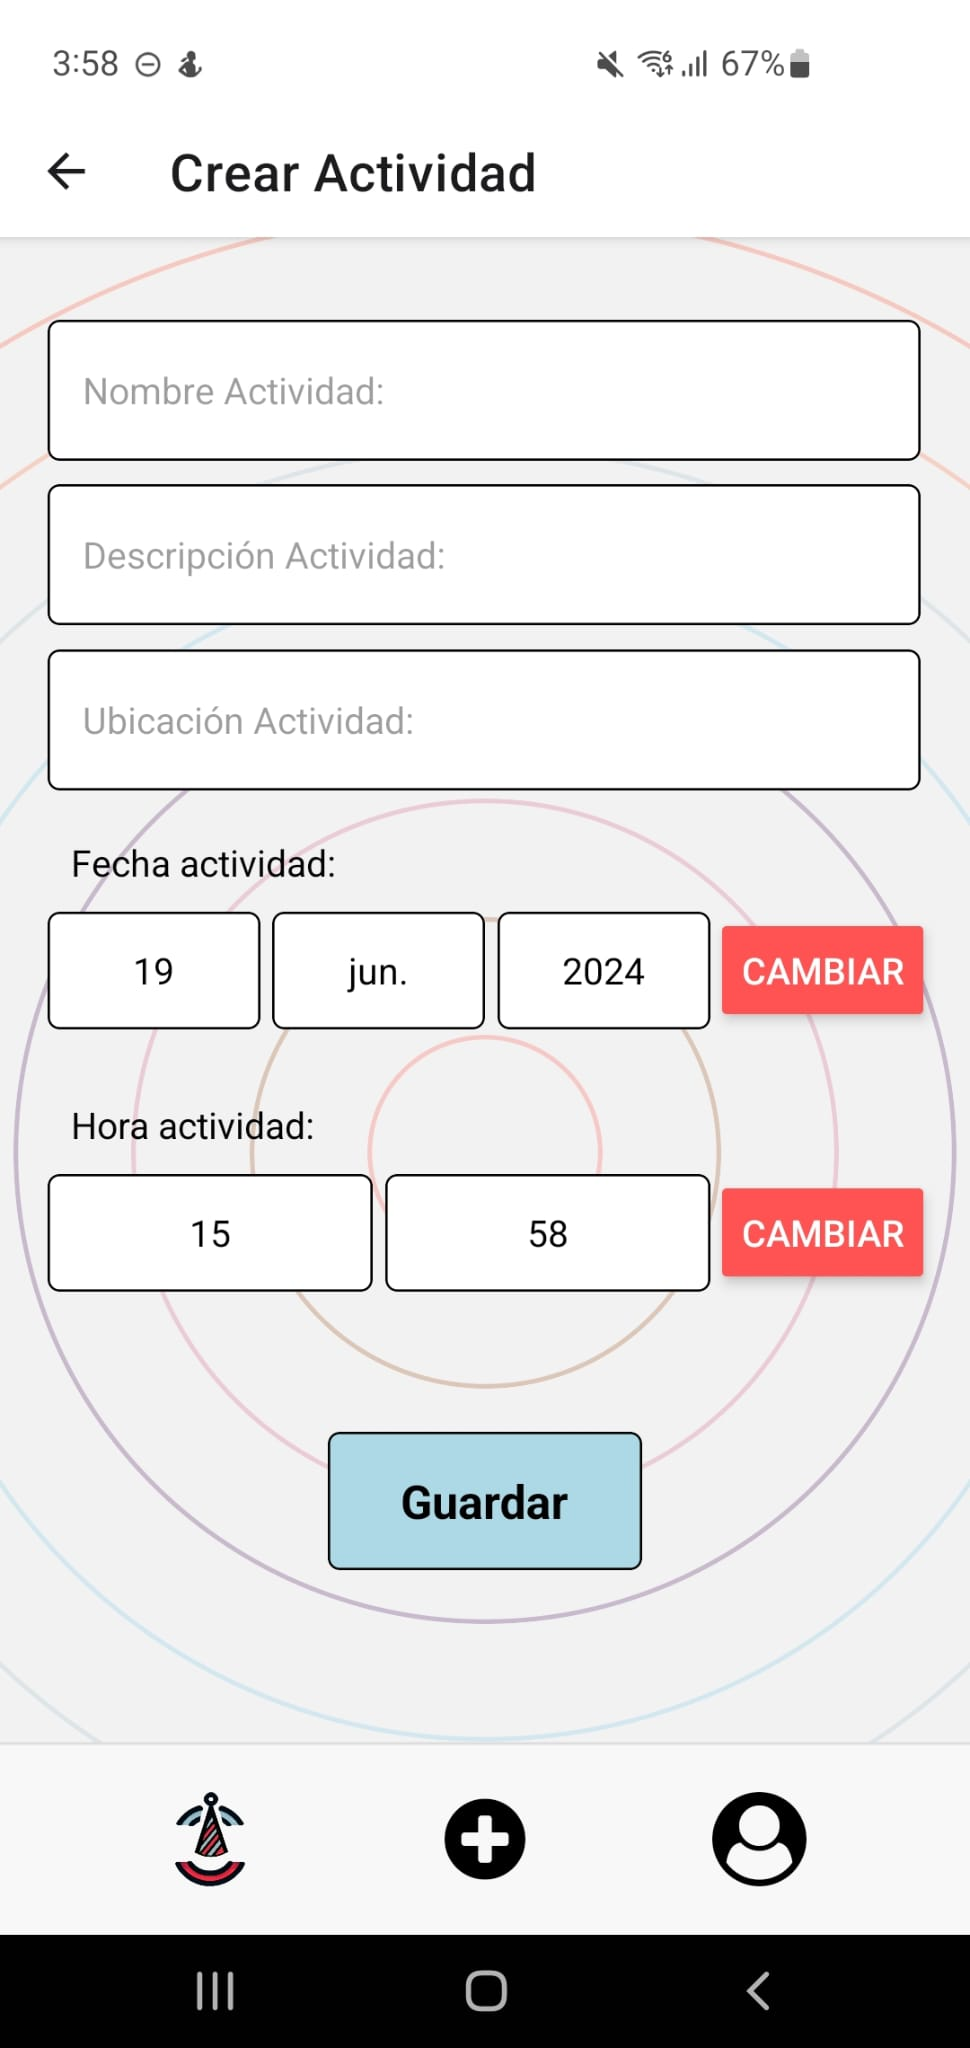
\includegraphics[width=\linewidth]{imagenes/Capturas/CrearActividad.jpeg}
        \caption{Crear Actividad}
        \label{fig:img5}
    \end{subfigure}%
    \hfill
    \begin{subfigure}{0.45\textwidth}
        \centering
        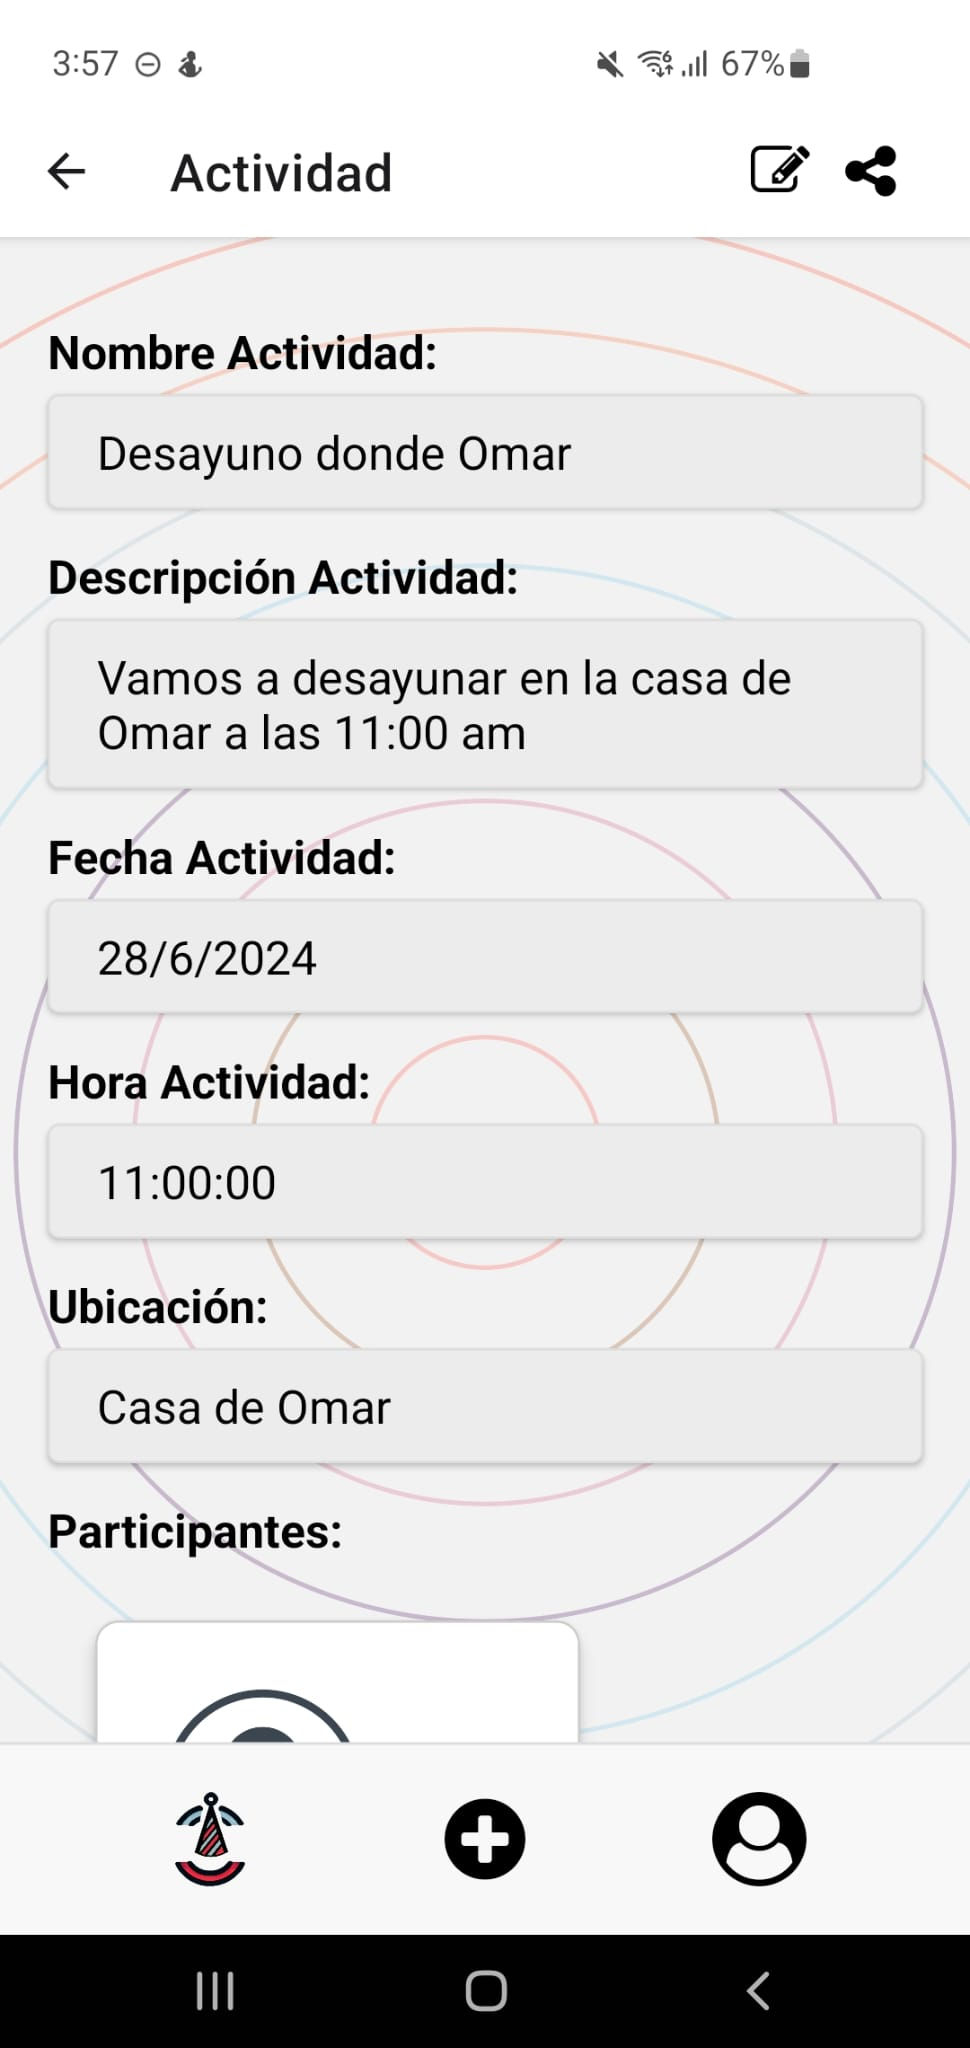
\includegraphics[width=\linewidth]{imagenes/Capturas/DatosActividad.jpeg}
        \caption{Datos de la Actividad}
        \label{fig:img6}
    \end{subfigure}
\end{figure}
\vspace*{\fill}

\clearpage
\vspace*{\fill}
\begin{figure}[H]
    \centering
    \begin{subfigure}{0.45\textwidth}
        \centering
        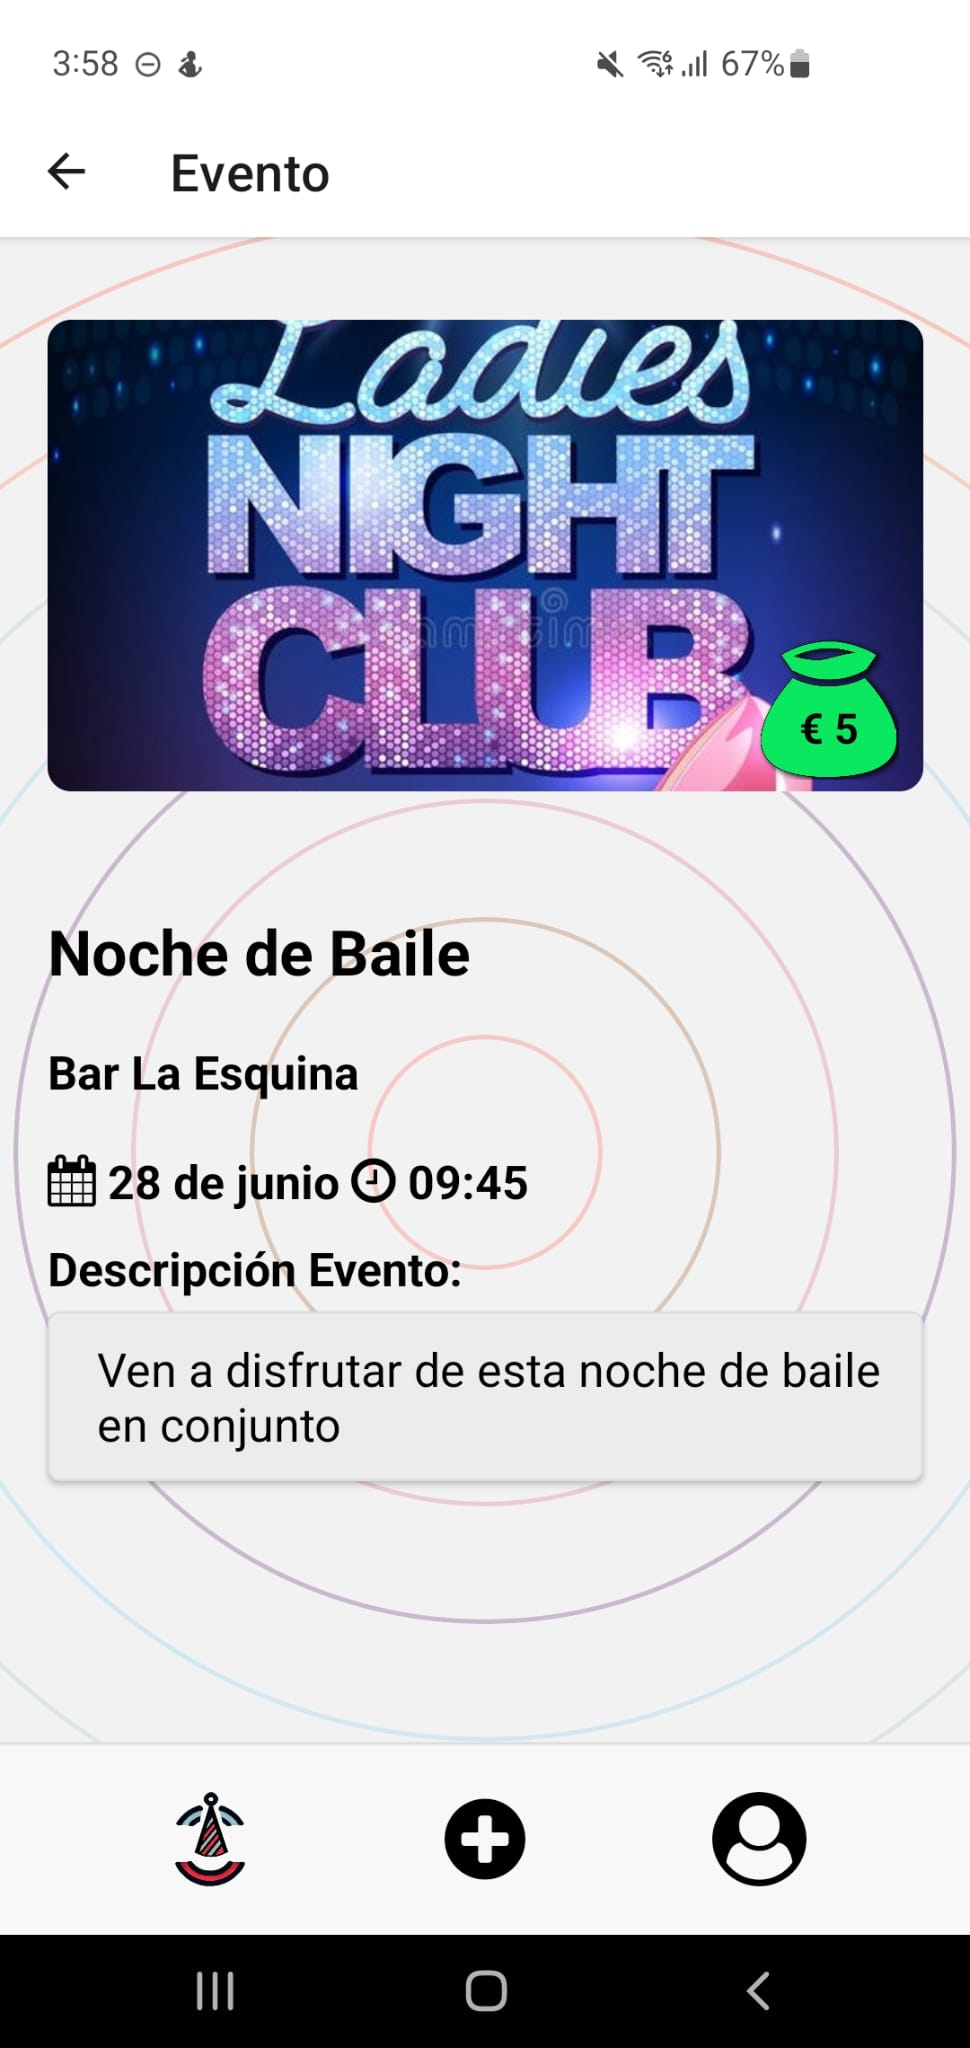
\includegraphics[width=\linewidth]{imagenes/Capturas/DatosEventoUsuario.jpeg}
        \caption{Datos de Evento}
        \label{fig:img5}
    \end{subfigure}%
    \hfill
    \begin{subfigure}{0.45\textwidth}
        \centering
        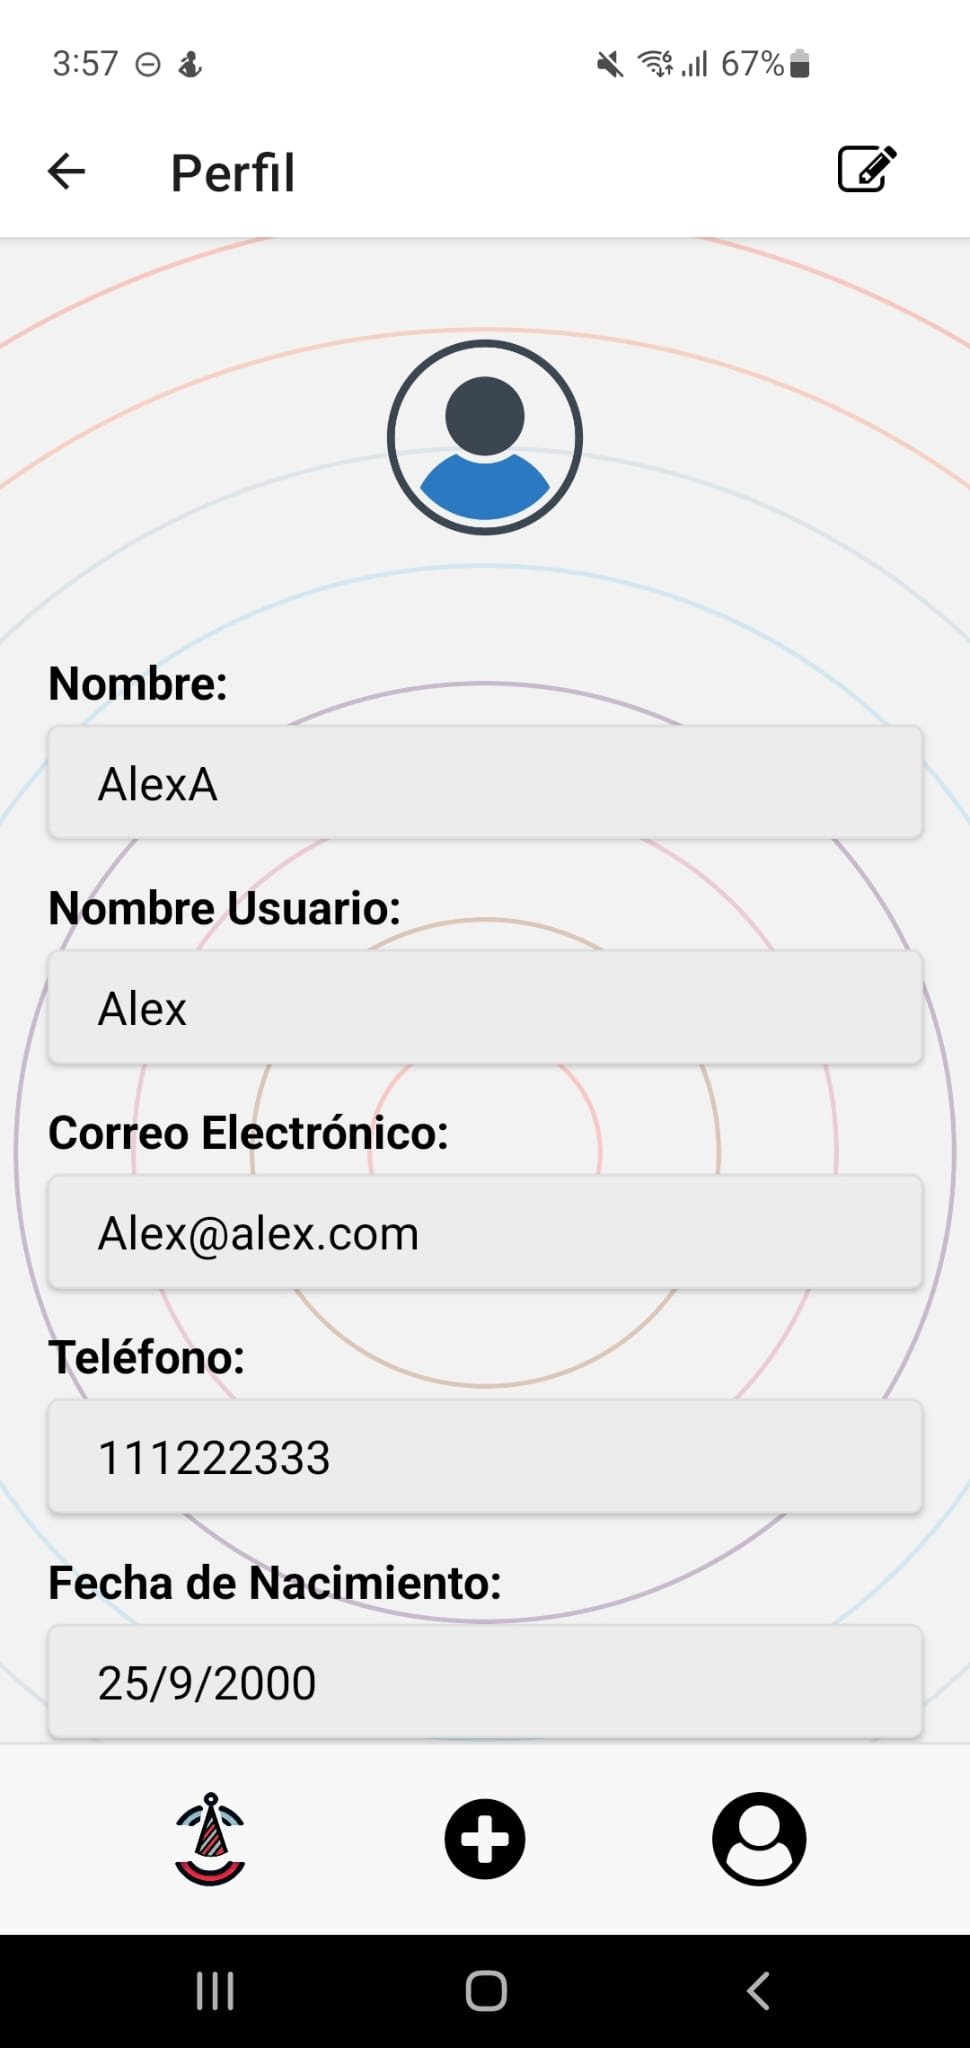
\includegraphics[width=\linewidth]{imagenes/Capturas/DatosPerfil.jpeg}
        \caption{Datos de Perfil}
        \label{fig:img6}
    \end{subfigure}
\end{figure}
\vspace*{\fill}

\subsection{Enlace a Vídeos}

En el siguiente enlace se pueden encontrar el vídeo del funcionamiento de la aplicación, divididos para mostrar la navegación del usuario y del administrador de establecimiento:

\href{https://youtu.be/Tzmj9JLn8yU}{Vídeo del funcionamiento de la aplicación}